\documentclass{article}

\usepackage[utf8]{inputenc}
\usepackage[spanish]{babel}

\usepackage{geometry}               % Márgenes del documento
\usepackage{amsfonts}
\usepackage{graphicx}

\usepackage{tabularx}

\usepackage{amsthm} % para teoremas y lemas

\usepackage[nottoc]{tocbibind}

\usepackage{color}
\usepackage[pdftex, colorlinks=true, linkcolor=blue, urlcolor=red, filecolor=magenta, citecolor=green]{hyperref}
\definecolor{gray97}{gray}{.97}
\definecolor{gray75}{gray}{.75}
\definecolor{gray45}{gray}{.45}

\usepackage{listings}
\usepackage[usenames,dvipsnames]{xcolor}
\colorlet{keyword}{blue!100!black!80}
\colorlet{STD}{Lavender}
\colorlet{comment}{green!80!black!90}

\lstdefinestyle{vhdl}{
	language     = VHDL,
	tabsize=3,
	numbers=left, % Donde se situan los numeros
	frame=single, % Se pone un marco
	backgroundcolor = \color{gray97},
	basicstyle   = \footnotesize \ttfamily,
	keywordstyle = [1]\color{keyword}\bfseries,
	keywordstyle = [2]\color{STD}\bfseries,
	breaklines=true,                % sets automatic line breaking
	commentstyle = \color{comment}
}

\lstdefinestyle{matlab}{
	language     = MATLAB,
	tabsize=3,
	numbers=left, % Donde se situan los numeros
	frame=single, % Se pone un marco
	backgroundcolor = \color{gray97},
	basicstyle   = \footnotesize \ttfamily,
	keywordstyle = [1]\color{keyword}\bfseries,
	keywordstyle = [2]\color{STD}\bfseries,
	breaklines=true,                % sets automatic line breaking
	commentstyle = \color{comment}
}

\geometry{a4paper}                  % Tamaño y márgenes del documento
\geometry{left=2.5cm,top=2.5cm}
\geometry{bottom=2.5cm,right=2.5cm}

\geometry{driver=dvips,pdftex} % ???
\setcounter{secnumdepth}{5}    % ???
\setcounter{tocdepth}{5}       % ???

%--------------------------------------------------------------------------
\title{\textbf{Prácticas de Sistemas en Tiempo Real} \\ Parte correspondiente a las prácticas de FPGAs}
\author{Francisco Abel Cedrón Santaeufemia \and \textit{francisco.cedron@udc.es}}
\date{} %Asi no inserta la fecha


\begin{document}


\maketitle % Pone titulo, autor

\renewcommand{\abstractname}{Abstract} % El nombre que aparece al principio del abstract
\begin{abstract}
En esta memoria correspondiente a la primera parte de prácticas de asignatura que se corresponde con al uso de FGAs de la asignatura de STR. En ella se podrá leer la solución a los boletines que hay para realizar.
\end{abstract}

\renewcommand{\contentsname}{} % Lo que pone en el indice
\tableofcontents

\vspace{2cm} % Para dejar un espacio con respecto a la tabla

\section{Práctica 2: Construcción de una ALU simple de 4 bits.}
\subsection{Enunciado.}
 Una ALU (\textit{Arithmetic Logic Unit}) es un circuito digital que lleva a cabo operaciones de aritmética entera (sumas, resta, multiplicaciones, divisiones), lógicas (AND, NOT, OR, XOR...) y de desplazamientos de bits. Su estructura puede verse en la figura \ref{fig:p2:alu}, donde A y B son los valores de entrada, R es el valor de salida, F indica la operación a realizar y D señala el estatus de la salida (acarreo de salida, overflow, división por cero...).

\begin{figure}[h]
  \centering
    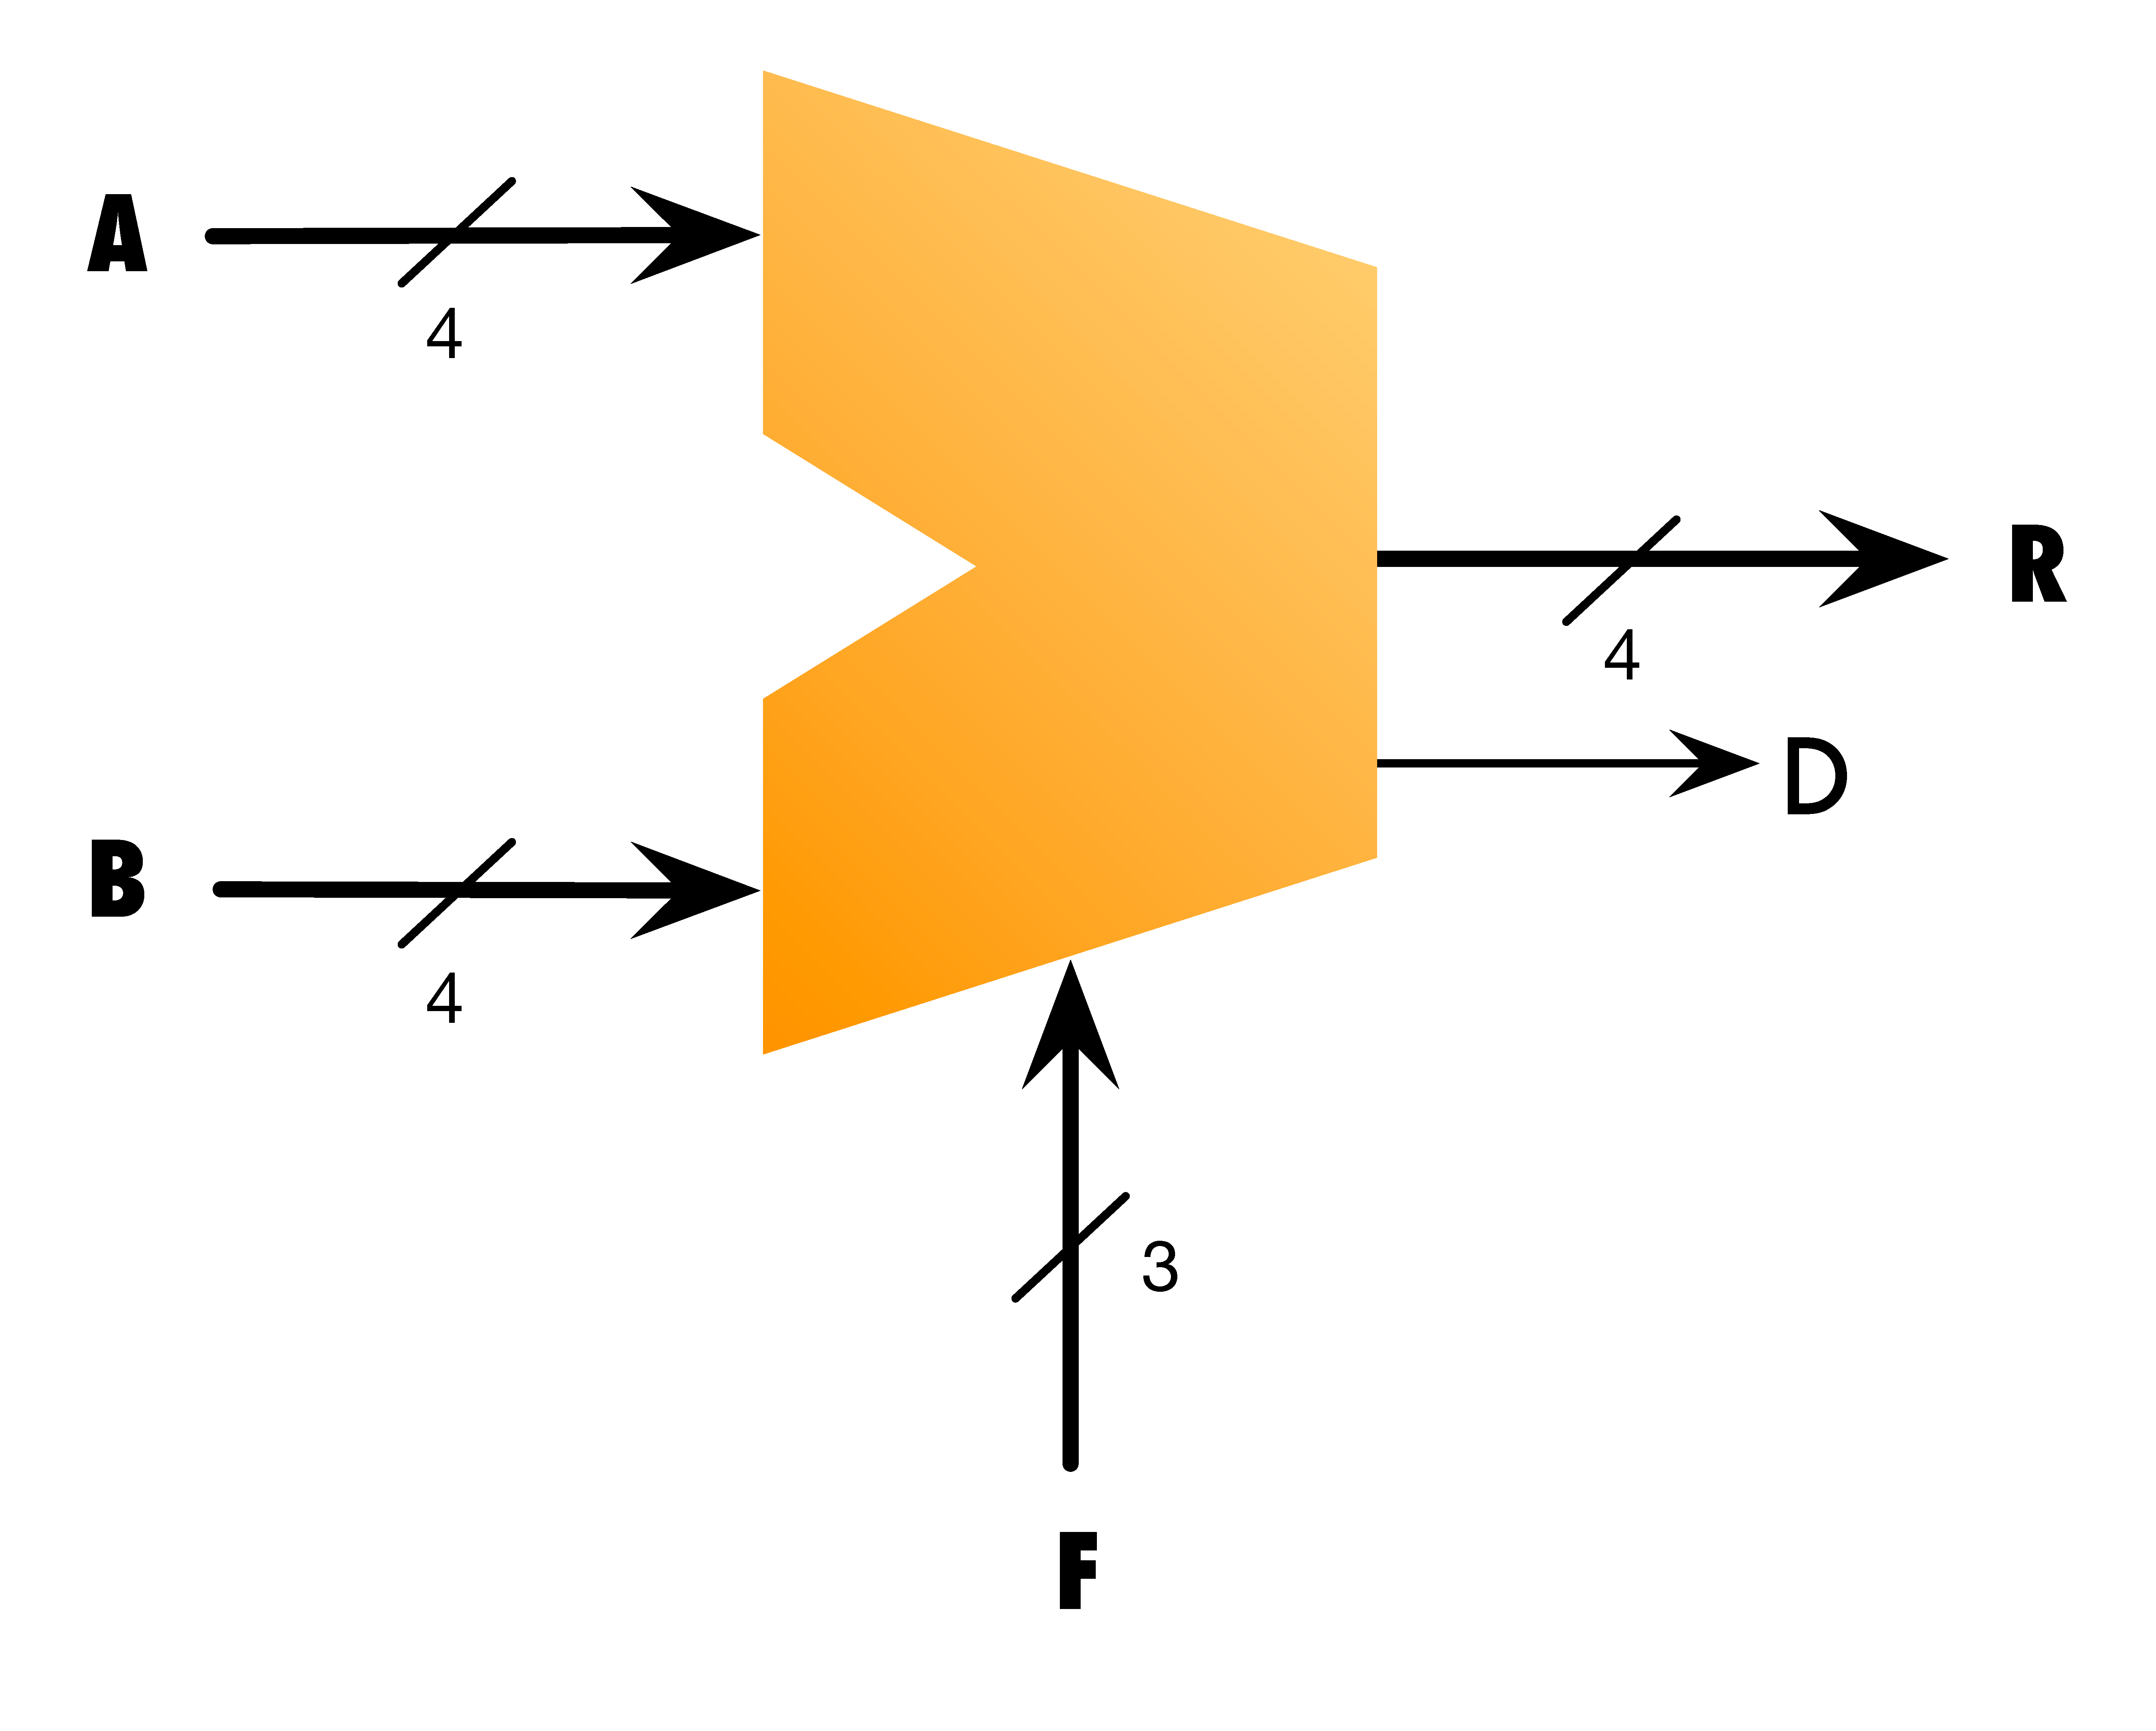
\includegraphics[width=0.3\textwidth]{img/ALU.pdf}
  \caption{Esquema de la ALU a implementar.}
  \label{fig:p2:alu}
\end{figure}

Se pide diseñar e implementar la estructura de ALU (entradas/salidas) teniendo en cuenta que se trabaja con registros de 4 bits. La ALU tiene que implementar las siguientes operaciones:
\begin{enumerate}
	\item NOT(A)
	\item AND
	\item OR
	\item XOR
	\item A + B
	\item A - B
	\item Desplazamiento de 1 bit a la izquierda de A
	\item Desplazamiento de 1 bit a la derecha de A
\end{enumerate}

\subsection{Implementación.}

Para comenzar con el diseño hay que definir los elementos de entrada y los elementos de salida
para ello identificamos las entradas que para el caso de la ALU (figura \ref{fig:p2:alu}) son los elementos \emph{A}, \emph{B} y \emph{F} y también tendremos como elemento de entrada la señal de reloj \emph{CLK}. Ahora nos queda identificar las salidas que en la ALU que estamos implementando son los elementos \emph{R} y \emph{D}.

En el enunciado se especifica que esta ALU trabaja con registros de 4 bits por eso los elementos \emph{A}, \emph{B} y \emph{R} aparecen como vectores de 4 elementos, mientras que la entrada \emph{F} tiene solamente 3 elementos que es el menos número de bits necesario para identificar las ocho operaciones que hará la ALU. La salida \emph{D} no es un vector porque solo se emplea para indicar si existe o no overflow en una operación. En la figura \ref{cod:p2:interfaz} se puede ver el código correspondiente con la interfaz de entrada.

\begin{figure}[h]
	\begin{lstlisting}[style=vhdl]
entity p2 is
	Port ( 
		A : in   STD_LOGIC_VECTOR (3 downto 0);
		B : in   STD_LOGIC_VECTOR (3 downto 0);
		F : in   STD_LOGIC_VECTOR (2 downto 0);
		R : out  STD_LOGIC_VECTOR (3 downto 0);
		D : out  STD_LOGIC;
		CLK : in STD_LOGIC);
end p2;
	\end{lstlisting}
	\caption{Definición de la interfaz.}
	\label{cod:p2:interfaz}
\end{figure}

Lo siguiente a realizar es proponer cuales cuales serán los códigos para cada operación. Para ello se ha creado la tabla
\ref{tab:p2:cod_operacion}
en donde se pueden ver la tabla donde especifica que código se corresponde con cada entrada.

\begin{table}
	\begin{center}
		\begin{tabular}{|c|c|}
\hline
\textbf{Código} & \textbf{Operación} \\ \hline
\hline
000 & NOT(A) \\ \hline
001 & A AND B\\ \hline
010 & A OR B \\ \hline
011 & A XOR B\\ \hline
100 & A + B  \\ \hline
101 & A - B  \\ \hline
110 & A $<$  1  \\ \hline
111 & A $>$   1  \\ \hline
		\end{tabular}
		\caption{Códigos de operación de la ALU.}
		\label{tab:p2:cod_operacion}
	\end{center}
\end{table}

Aunque el enunciado no lo especifique se ha incluido una señal de reloj \emph{CLK} para poder tener las operaciones sincronizadas. Esa señal de reloj \emph{CLK} se ha añadido a la lista de sensibilidad del proceso y se ha controlado que esa sincronización se hace en el flanco de bajada del reloj con la operación haciendo uso de
\begin{enumerate}
	\item \emph{CLK'EVENT} que devuelve true si existe un cambio en la señal de reloj.
	\item \emph{CLK = '0'} es la comprobación de que la señal está en el flanco negativo.
\end{enumerate}
En la figura \ref{cod:p2:process} se puede ver el código del proceso que implementa la lógica de la ALU.

\begin{figure}[h]
	\begin{lstlisting}[style=vhdl]
PROCESS (CLK)
begin
	IF CLK'EVENT AND CLK='0' THEN
		D <= '0';
		CASE F IS
			WHEN "000"  =>
				R <= not A;
			WHEN "001"  => 
				R <= A and B;
			WHEN "010"  =>
				R <= A or B;
			WHEN "011"  =>
				R <= A xor B;
			WHEN "100"  =>
				R <= A + B;
				D <= A(3) and B(3);
			WHEN "101"  => 
				R <= A - B;
			WHEN "110"  =>
				R <= (A(2 downto 0) & '0');
			WHEN "111"  =>
				R <= ('0' & A(3 downto 1));
			WHEN OTHERS =>
				R <= A;
		END CASE;
	END IF;

end process;
	\end{lstlisting}
	\caption{Proceso que implementa las operaciones de la ALU.}
	\label{cod:p2:process}
\end{figure}

\subsection{Test.}

Para poder comprobar el funcionamiento de nuestra ALU se ha simulado su comportamiento creando un \emph{Test Bench}. Dicha simulación se muestra en la figura \ref{fig:p2:tb} y a continuación se explica las pruebas realizadas en ella.

\begin{enumerate}
	\item Se empieza estableciendo el valor de \emph{A} a \emph{1000} con la función \emph{F = 000} que se corresponde con la función \emph{NOT(A)}. Se puede ver que el resultado \emph{R} es \emph{0111}.
	\item Se establecen los valores de \emph{A} a \emph{1110} y \emph{B} a \emph{0111} y se realiza la función \emph{A and B} que se corresponde con el código \emph{F = 001}. El resultado de la operación es \emph{0110} que es el que tiene la salida \emph{R}.
	\item Con los valores de \emph{A} y \emph{B} anteriores (1110 y 0111 respectivamente) se realiza la operación \emph{A or B} (que se corresponde con el código \emph{F = 010}. El resultado \emph{1110 or 0111} es \emph{1111} que es el mismo que tiene la salida \emph{R}.
	\item Continuando con los valores anteriores para \emph{A} y \emph{B} se procede a probar la operación \emph{xor}, con lo que \emph{R} tiene el resultado de \emph{1110 xor 0111} que es \emph{1001}.
	\item Se establece los valores \emph{1011} y \emph{1010} para \emph{A} y \emph{B} respectivamente y se procede a probar la suma (que se corresponde con el código \emph{F = 100}. El resultado de la suma \emph{1011 + 1010} es \emph{10101} (que en decimal se corresponde con \emph{11 + 10 = 21}. Para representar este resultado se necesitan 5 bits pero los registros son de 4 bits, por eso se ve que el registro \emph{R} tiene el valor \emph{0101}. Esta situación se corresponde con lo que se conoce como \emph{overflow} y es lo que indica en ese momento la línea \emph{D} al estar activada.
	\item Ahora se procede con la prueba de la resta (\emph{F = 101}) con los valores de \emph{A} y \emph{B} que se emplearon en la prueba del paso anterior. Con esto tenemos que la resta de \emph{1011 - 1010 = 0001} que es exactamente lo mismo que hay en el elemento \emph{R}.
	\item  Para poder probar la operación de desplazamiento a la izquierda se emplea el código \emph{F = 110} con el valor \emph{1011} para el registro \emph{A}. El resultado de esa operación es \emph{0110}.
	\item La última operación que queda por realizar es el desplazamiento de un bit a la derecha por eso se establece el valor de la función \emph{F} a \emph{111}. El registro \emph{R} tiene el valor \emph{0101} que es exactamente el que se corresponde con la operación \emph{1011 $>$ 1}.
\end{enumerate}


\begin{figure}[h]
  \centering
    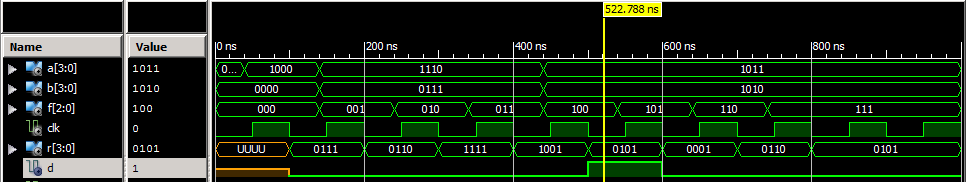
\includegraphics[width=1\textwidth]{img/p2_tb.png}
  \caption{Resultados obtenidos en la ALU al realizar la simulación.}
  \label{fig:p2:tb}
\end{figure}

\section{Práctica 3: Construcción de un microprocesador simple.}

\subsection{Enunciado.}

Un microprocesador es un circuito constituido básicamente por registros y una ALU. Aunque un microprocesador recibe las instrucciones en binario, en esta práctica se va a suponer que las instrucciones se reciben en ensamblador. En concreto se podrá recibir cualquier de las siguientes instrucciones:
\begin{itemize}
	\item \emph{lda $<$valor$>$}: carga \emph{$<$valor$>$} en el acumulador \emph{A}.
	\item \emph{lda $<$valor$>$}: carga \emph{$<$valor$>$} en el acumulador \emph{B}.
	\item \emph{add}: suma los valores de los acumuladores \emph{A} y \emph{B}.
	\item \emph{sub}: resta el contenido de los acumuladores \emph{A} y \emph{B}
	\item \emph{seta $<$dir$>$}: coloca el valor del acumulador \emph{A} en la posición \emph{$<$dir$>$} del registro.
	\item \emph{setb $<$dir$>$}: coloca el valor del acumulador \emph{B} en la posición \emph{$<$dir$>$} del registro.
	\item \emph{outa}: coloca el acumulador \emph{A} en la salida de datos.
	\item \emph{xrc}: intercambia el contenido de los acumuladores \emph{A} y \emph{B}.
\end{itemize}

Con este conjunto de instrucciones será necesario que el microprocesador posea: una entrada para instrucciones, una entrada para datos, una salida de datos, una entrada para direcciones, dos acumuladores (\emph{A} y \emph{B}) y un registro con 256 posiciones para enteros.

El diseño y la implementación de la estructura del microprocesador debe tener en cuenta que los operandos, registros y acumuladores son de tipo entero. A mayores se pide que el comportamiento del micropocesador use el tipo enumerado comprendiendo todas las instrucciones posibles y que efectúe para cada una de éstas las operaciones correspondientes.

\subsection{Implementación.}

Para implementar las instrucciones del microprocesador se ha usado un tipo enumerado. Dicho tipo se ha defenido en un paquete para que pueda ser usado en la \emph{entity} donde se define las entradas y salidas de la FPGA. El contenido del paquete es el que se muestra en la figura \ref{cod:p3:package}. Como se puede ver en la figura \ref{cod:p3:package} el paquete también contiene la definición de un tipo llamado \emph{TYPE\_REGISTER} el cual es un array de enteros con 256 posiciones. Este tipo de dato será empleado para implementar la memoria del microprocesador.


\begin{figure}[h]
	\begin{lstlisting}[style=vhdl]
PACKAGE types IS
	TYPE TYPE_INSTRUCTIONS IS (lda, ldb, add, sub, seta, setb, outa, xcr);
	TYPE TYPE_REGISTER     IS ARRAY (255 DOWNTO 0) OF INTEGER;
END types;
	\end{lstlisting}
	\caption{Paquete con definición de nuevos tipos.}
	\label{cod:p3:package}
\end{figure}

Antes de empezar con a implementar la lógica necesaria para está práctica hay que definir las entradas y salidas de la FPGA acorde con el enunciado. En la figura \ref{cod:p3:entity} se puede ver que las a excepción del reloj (\emph{CLK}) y de las instrucciones del microprocesador (\emph{INSTRUCTION}) los tipos de datos son todos de tipo entero.

\begin{figure}[h]
	\begin{lstlisting}[style=vhdl]
entity p3 is
    Port ( CLK        : in  STD_LOGIC;
           INSTRUCTION: in  TYPE_INSTRUCTIONS;
           INPUT      : in  INTEGER;
           A          : out INTEGER;
           B          : out INTEGER;
           ADDRESS    : in  INTEGER;
           OUTPUT     : out INTEGER
         );
end p3;
	\end{lstlisting}
	\caption{Definición de la interfaz.}
	\label{cod:p3:entity}
\end{figure}

El procesador entero de la FPGA se simula como un proceso cuya lista de sensibilidad es la señal de entrada del reloj (\emph{CLK}) y sólo realiza las operaciones en el flanco positivo de la señal de reloj. El código correspondiente al proceso que implementa el comportamiento del microprocesador se puede ver en la figura \ref{cod:p3:process}.

\begin{figure}[h]
	\begin{lstlisting}[style=vhdl]
process (CLK)
	VARIABLE tmpA: INTEGER;
	VARIABLE tmpB: INTEGER;
	VARIABLE reg:  TYPE_REGISTER;
	VARIABLE tmp:  INTEGER;
begin
	if CLK='1' and CLK'event then
		case (instruction) is
			when lda    => tmpA := INPUT;        -- cargar en el acumulador A
			when ldb    => tmpB := INPUT;        -- cargar en el acumulador B
			when add    => tmpA := tmpA + tmpB;  -- sumar acumulador A y el B
			when sub    => tmpA := tmpA - tmpB;  -- restar acumulador A menos el B
			when seta   => reg(ADDRESS) := tmpA; -- guarda el acumulador A en ADDRESS
			when setb   => reg(ADDRESS) := tmpB; -- guarda el acumulador B en ADDRESS
			when outa   => OUTPUT <= tmpA;       -- pone en la salida el acumulador A
			when xcr    => tmp  := tmpA;         -- intercambia el contenido de los acumuladores
								tmpA := tmpB;
								tmpB := tmp;
			when others => NULL; -- otra cosa: no se hace nada
		end case;
		A <= tmpA;
		B <= tmpB;
	end if;
end process;
	\end{lstlisting}
	\caption{Implementación de la lógica de un microprocesador simple.}
	\label{cod:p3:process}
\end{figure}

\subsection{Test.}

	Para poder comprobar el correcto funcionamiento del procesador se ha desarrollado un \emph{Test Bench}. Los operaciones que se han realizado han sido:
	
\begin{enumerate}
	\item Se asigna un \emph{5} a la entrada y se almacena en el acumulador \emph{A}.
	\item Se asigna un \emph{2} a la entrada y se almacena en el acumulador \emph{B}.
	\item Se suma el valor de los acumuladores \emph{A} y \emph{B} y el resultado se almacena en el acumulador \emph{A}. Ahora el valor de \emph{A} es \emph{7}.
	\item Se resta el valor del acumulador \emph{B} al del \emph{A} y el resultado se almacena en el acumulador \emph{A}. Ahora en el elemento \emph{A} está el valor \emph{5}.
	\item Se almacena el valor del acumulador \emph{A} en el registro \emph{0}.
	\item Se almacena el valor del acumulador \emph{B} en el registro \emph{10}.
	\item Se almacena el valor del acumulador \emph{A} en la salida (\emph{OUTPUT}).
	\item Se intercambian los valores de los acumuladores.
	\item Se almacena el valor del acumulador \emph{A} en la salida (\emph{OUTPUT}).
\end{enumerate}

Como se puede comprobar en la figura \ref{fig:p3:tb} el microprocesador muestra los resultados esperados. El resultado de los pasos 5 y 6 no se puede ver porque la memoria del microprocesador está implementada como una variable y  el contenido de las variables no puede ser monitorizado.

\begin{figure}[h]
  \centering
    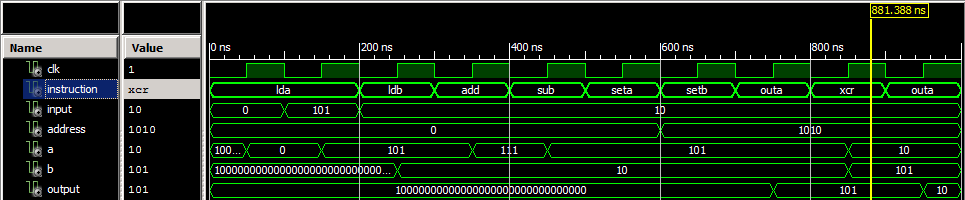
\includegraphics[width=1\textwidth]{img/p3_tb.png}
  \caption{Resultados obtenidos en la simulación del microprocesador.}
  \label{fig:p3:tb}
\end{figure}


\section{Práctica 4: ECU Simple para Control de Estabilidad y Airbags.}

\subsection{Enunciado.}

Una ECU (\emph{Electronic Control Unit}) es un hardware embebido que se encarga de controloar uno o varios subsistemas eléctricos de un vehículo. En esta práctica denominaremos ECU al sistema encargado de controlar los airbags y el sistema de estabilidad de un coche (aunque realmente los coches de hoy en día llevan varias ECUs).

Nuestra ECU recibirá información de los siguientes sensores:
\begin{itemize}
	\item \textbf{Acelerómetro}. Utilizado para determinar cuándo se produce una colisión. Mientras no se detecte ésta, mandará periódicamente el mensaje \emph{acelcero}. En cuanto se detecte un impacto enviará el mensaje \emph{aceluno}.
	\item \textbf{Sensores de presión de puertas}. Sirven para detectar cuándo se produce una colisión lateral. Si se detecta dicha colisión, enviará un mensaje \emph{presXuno}. En caso contrario, enviará periódicamente el mensaje \emph{presXcero}. Para simplificar la práctica, se supone que tan sólo hay dos sensores de este tipo, uno para la puerta del conductor y otro para la del acompañante.
	\item \textbf{Sensor de acompañante}. Permite determinar si existe en el vehículo alguien que esté ocupando el puesto de copiloto. En caso positivo, enviará el mensaje \emph{ocupuno} y en caso negativo, \emph{ocupcero}.
	\item \textbf{Sensor de velocidad de las ruedas}. Miden la velocidad de rotación de las ruedas. Para simplificar se supone que este sensor sólo envía información de una rueda si ésta gira más deprisa (\emph{ruedaXuno}), más lento (\emph{ruedaXdos}) o igual de rápido que las demás (\emph{ruedaXcero}). Se controlarian entonces las cuatro ruedas del coche.
\end{itemize}

En función de los mensajes recibidos, la ECU realizará dos tareas: la ignición de los airbags y la regulación de la presión hidráulica de los frenos.

Se asume que existen cuatro airbags en el coche: dos frontales y dos laterales. Para que el airbag sea efectivo, su despliegue debe realizarse en un tiempo inferior a 60 ms que se reparten de la siguiente manera:
\begin{itemize}
	\item 30 ms se gastan en el inflado
	\item 2 ms en la ignición
	\item quedan 28 ms como máximo para dedicar en la detección de la colisión
\end{itemize}

Con respecto al sistema de estabilidad, la regulación de la presión hidráulica se realizará sobre cada una de las cuatro válvulas que hay en el sistema de frenado.

Para interactuar con todos estos elementos la ECU hará uso de señales que se muestran en la tabla
\ref{tab:p4:salida_ECU}.

\begin{table}[H]
    \centering
    \begin{tabularx}{\textwidth}{| c | X |}
        \hline
\textbf{Señal de salida (valor inicial = 0)} & \textbf{Instante de activación (valor = 1)}     \\ \hline
\emph{IGNICION\_AIRBAG\_FRONTAL\_CONDUCTOR} & Impacto en el vehículo (sea lateral o no) \\ \hline
\emph{IGNICION\_AIRBAG\_FRONTAL\_ACOMP} & Impacto (lateral o no) cuando existe un acompañante.\\ \hline
\emph{IGNICION\_AIRBAG\_LATERALES} & Cuando se detecte una colisión lateral (exista o no acompañante) \\ \hline
\emph{REDUCE\_PRESION\_HIDRAULICA} & Cuando se detecta que la rueda gira más lenta que las demás ruedas\\ \hline
\emph{AUMENTA\_PRESION\_HIDRAULICA} & Cuando se detecta que la rueda gira más rápido que las otras ruedas  \\ \hline
    \end{tabularx}
	\caption{Señales de salida de la ECU.}
	\label{tab:p4:salida_ECU}
\end{table}

Con esto el funcionamiento de la ECU sería el siguiente:
\begin{itemize}
	\item \textbf{Sistema de Airbags:}
	\begin{enumerate}
		\item La ECU monitoriza el acelerómetro, el sensor de presión de las puertas y el de presencia del acompañante.
		\item Si el acelerómetro indica que se ha producido un impacto, se activará la ignición de los airbags frontales y laterales en función del valor del sensor de ocupación y de los sensores de presión de las puertas.
	\end{enumerate}
	
	\item \textbf{Sistema de estabilidad:}
	\begin{enumerate}
		\item La ECU controla constantemente la velocidad de rotación de cada rueda.
		\item Si una de las ruedas gira más rápido que las demás, se aumenta la presión hidráulica sobre dicha rueda.
		\item Si una rueda gira más lento que las demás, se reduce la presión hidráulica sobre la misma.
	\end{enumerate}
\end{itemize}

Para el diseño y la implementación de la estructura de la ECU es necesario crear un \emph{tipo de mensaje} para la entrada y que las señales de salida son de tipo \emph{STD\_LOGIC.}

\subsection{Implementación.}

	Lo primero que se ha decidido es generar los mensajes que puede recibir la ECU a través de los subsistemas. Para ello se han usado tipos enumerados que se han definido en un paquete para que pueda ser usado en la \emph{entity} donde se definen las entradas y salidas de la FPGA. El contenido del paquete es el que se muestra en la figura \ref{cod:p4:package}. Como se puede apreciar en la figura \ref{cod:p4:package} el paquete contiene dos tipos de arrays \emph{A\_MSG\_DOOR} y \emph{A\_MSG\_WHEEL} los cuales reciben por un bus los mensajes de los sensores de presión de las puertas y los sensores de velocidad de las ruedas respectivamente.

\begin{figure}[h]
	\begin{lstlisting}[style=vhdl]
PACKAGE types IS
	TYPE T_MSG_ACCELEROMETER IS (acelcero, aceluno);
	TYPE T_MSG_DOOR          IS (prescero, presuno);
	TYPE A_MSG_DOOR          IS ARRAY (0 TO 1) OF T_MSG_DOOR;
	TYPE T_MSG_ACCOMPANIST   IS (ocupcero, ocupuno);
	TYPE T_MSG_WHEEL         IS (ruedacero, ruedauno, ruedados);
	TYPE A_MSG_WHEEL         IS ARRAY (0 TO 3) OF T_MSG_WHEEL;
END types;
	\end{lstlisting}
	\caption{Paquete con definición de nuevos tipos.}
	\label{cod:p4:package}
\end{figure}

Antes de empezar con a implementar la lógica necesaria para está práctica hay que definir las entradas y salidas de la FPGA acorde con el enunciado. En la figura \ref{cod:p4:entity} se muestra el código correspondiente a ello.

\begin{figure}[h]
	\begin{lstlisting}[style=vhdl]
    Port ( CLK : in STD_LOGIC;
			  -- SENALES DE SALIDA PARA LAS RUEBAS
	        -- SE USAN BUS DONDE LA POSICION 0 ES LA RUEBA A, 1 LA RUEDA B, ETC
			  REDUCE_PRESION_HIDRAULICA  : out  STD_LOGIC_VECTOR (3 downto 0);
			  AUMENTA_PRESION_HIDRAULICA : out  STD_LOGIC_VECTOR (3 downto 0);
           -- SENALES DE SALIDA PARA LOS AIRBAGS
			  IGNICION_AIRBAG_FRONTAL_CONDUCTOR : out  STD_LOGIC;
           IGNICION_AIRBAG_FRONTAL_ACOMP     : out  STD_LOGIC;
           IGNICION_AIRBAGS_LATERALES        : out  STD_LOGIC;
           -- ENTRADAS PARA EL CONTROL DE LOS AIRBAGS
           MSG_ACCELEROMETER : in  T_MSG_ACCELEROMETER;
           MSG_DOOR          : in  A_MSG_DOOR;
           MSG_ACCOMPANIST   : in  T_MSG_ACCOMPANIST;
           -- ENTRADAS PARA EL CONTROL DE LAS RUEBAS
			  MSG_WHEEL : in  A_MSG_WHEEL);
	\end{lstlisting}
	\caption{Definición de las entradas y salidas que usará la ECU.}
	\label{cod:p4:entity}
\end{figure}

Para facilitar la lectura del proceso que se encarga de implementar el comportamiento de la ECU se han declarado una serie de funciones que se declaran en la \emph{entity}. Estas funciones son para saber que airbags activar y sobre que ruedas hay que actuar. Estas funciones se pueden ver en las figuras \ref{cod:p4:airbag_frontal_cond}, \ref{cod:p4:airbag_frontal_acomp}, \ref{cod:p4:airbags_laterales}, \ref{cod:p4:reduce_presion} y \ref{cod:p4:aumenta_presion}.

Gracias al uso de las funciones que aparecen en las figuras
\ref{cod:p4:airbag_frontal_cond}, \ref{cod:p4:airbag_frontal_acomp}, \ref{cod:p4:airbags_laterales}, \ref{cod:p4:reduce_presion} y \ref{cod:p4:aumenta_presion}
el código del proceso que controla el funcionamiento de la ECU queda muy legible. En la figura \ref{cod:p4:process} se puede ver la lógica que sigue la ECU, cuyo proceso tiene la señal de reloj (\emph{CLK}) en la lista de sensibilidad y sólo realiza las operaciones en el flanco positivo de la señal (ese comportamiento se consigue llamando a la función \emph{rising\_edge(CLK)}).

\begin{figure}[h]
	\begin{lstlisting}[style=vhdl]
FUNCTION airbag_frontal_cond(a: T_MSG_ACCELEROMETER; d: A_MSG_DOOR)
RETURN STD_LOGIC IS
  VARIABLE result: STD_LOGIC := '0';
BEGIN
	if (a = aceluno) then
		return '1';
	end if;
	
	for i in 0 to (d'LENGTH - 1) LOOP
		if (d(i) = presuno) then
			return '1';
		end if;
	end loop;
	
	return '0';

end airbag_frontal_cond;
	\end{lstlisting}
	\caption{Función para saber si el airbag frontal del conductor se tiene que activar.}
	\label{cod:p4:airbag_frontal_cond}
\end{figure}

\begin{figure}[h]
	\begin{lstlisting}[style=vhdl]
FUNCTION airbag_frontal_acomp(a:T_MSG_ACCELEROMETER; d:A_MSG_DOOR; p:T_MSG_ACCOMPANIST)
RETURN STD_LOGIC IS
  VARIABLE result: STD_LOGIC := '0';
BEGIN
	if (p = ocupcero) then
		return '0';
	else
		return airbag_frontal_cond(a,d);
	end if;
end airbag_frontal_acomp;
	\end{lstlisting}
	\caption{Función para saber si el airbag del copiloto se tiene que activar.}
	\label{cod:p4:airbag_frontal_acomp}
\end{figure}	

\begin{figure}[h]
	\begin{lstlisting}[style=vhdl]
FUNCTION airbags_laterales(d:A_MSG_DOOR)
RETURN STD_LOGIC IS
  VARIABLE result: STD_LOGIC := '0';
BEGIN
	for i in 0 to (d'LENGTH - 1) LOOP
		if (d(i) = presuno) then
			return '1';
		end if;
	end loop;
	
	return '0';	
end airbags_laterales;
	\end{lstlisting}
	\caption{Función para saber si los airbags laterales se tienen que activar.}
	\label{cod:p4:airbags_laterales}
\end{figure}

\begin{figure}[h]
	\begin{lstlisting}[style=vhdl]
FUNCTION reduce_presion(w:A_MSG_WHEEL)
RETURN STD_LOGIC_VECTOR IS
  VARIABLE result: STD_LOGIC_VECTOR(3 downto 0);
BEGIN
	for i in 0 to 3 loop
		if (w(i) = ruedados) then
			result(i) := '1';
		else
			result(i) := '0';
		end if;
	end loop;
	return result;
end reduce_presion;
	\end{lstlisting}
	\caption{Función para saber si se necesita reducir la presión hidraulica de alguna rueda.}
	\label{cod:p4:reduce_presion}
\end{figure}

\begin{figure}[h]
	\begin{lstlisting}[style=vhdl]
FUNCTION aumenta_presion(w:A_MSG_WHEEL)
RETURN STD_LOGIC_VECTOR IS
  VARIABLE result: STD_LOGIC_VECTOR(3 downto 0);
BEGIN
	for i in 0 to 3 loop
		if (w(i) = ruedauno) then
			result(i) := '1';
		else
			result(i) := '0';
		end if;
	end loop;
	return result;
end aumenta_presion;
	\end{lstlisting}
	\caption{Función para saber si se necesita aumentar la presión hidráulica de alguna rueda.}
	\label{cod:p4:aumenta_presion}.
\end{figure}

\begin{figure}[h]
	\begin{lstlisting}[style=vhdl]
process (CLK) begin
	if (rising_edge(CLK)) then
		-- airbag
		IGNICION_AIRBAG_FRONTAL_CONDUCTOR <= airbag_frontal_cond (MSG_ACCELEROMETER, MSG_DOOR);
		IGNICION_AIRBAG_FRONTAL_ACOMP     <= airbag_frontal_acomp(MSG_ACCELEROMETER, MSG_DOOR,
		                                                          MSG_ACCOMPANIST);
		IGNICION_AIRBAGS_LATERALES        <= airbags_laterales   (MSG_DOOR);
		-- ruedas
		REDUCE_PRESION_HIDRAULICA  <= reduce_presion (MSG_WHEEL);
		AUMENTA_PRESION_HIDRAULICA <= aumenta_presion(MSG_WHEEL);
	end if;
end process;
	\end{lstlisting}
	\caption{Implementación usada para definir el comportamiento de la ECU.}
	\label{cod:p4:process}
\end{figure}

\subsection{Test.}

Para poder comprobar el como se comporta la ECU se ha decidido simular su comportamiento y para ello se generaron un \emph{Test Bench} para comprobar su funcionamiento. Lo que también se modifico fue la frecuencia de tiempo para asegurarse de que no tarde más de 28 milisegundos. Para ello el tiempo que se escogió como periodo de la señal de reloj fue de 14 milisegundos para asegurarnos de que si se recibe el impacto poco después de que se produzca el flanco positivo de la señal de reloj pueda ser ejecutado en el siguiente flanco positivo y se puedan cumplir los 28 milisegundos. En realidad se podría escoger cualquier periodo que fuese inferior a 14 milisegundos
\footnote{Siempre y cuando en el periodo de la señal de reloj se puedan ejecutar todas las operaciones.}
. La decisión de dejarlo a 14 milisegundos es por el motivo de \emph{underclock} lo que ayuda a reducir la temperatura de los componentes y el consumo eléctrico.

Para poder ver mejor los resultados de la simulación se ha dividido el \emph{Test Bench} en dos partes, una para la comprobación de los airbags y la otra para la comprobación de estabilidad. Para cambiar de un modo a otro se ha creado una variable dentro del proceso \emph{stim\_proc} llamada \emph{prove\_airbag} de tal manera que si está a \emph{true} se prueban los airbags (figura \ref{fig:p4:tb_airbag}) y se establece a \emph{false} se prueba el control de estabilidad (figura  \ref{fig:p4:tb_wheel}).

\begin{figure}[h]
  \centering
    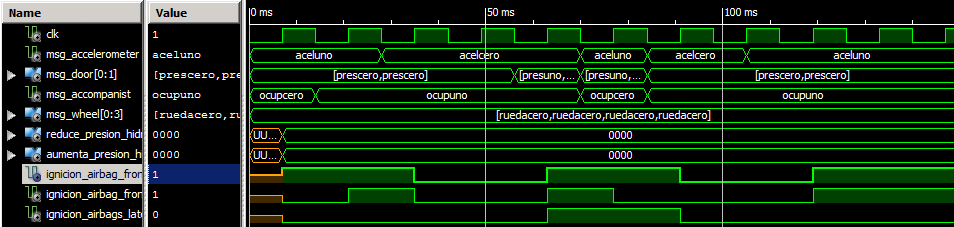
\includegraphics[width=1\textwidth]{img/p4_tb_airbag.png}
  \caption{Resultado obtenido en la simulación de la ECU al probar los airbags.}
  \label{fig:p4:tb_airbag}
\end{figure}

\begin{figure}[h]
  \centering
    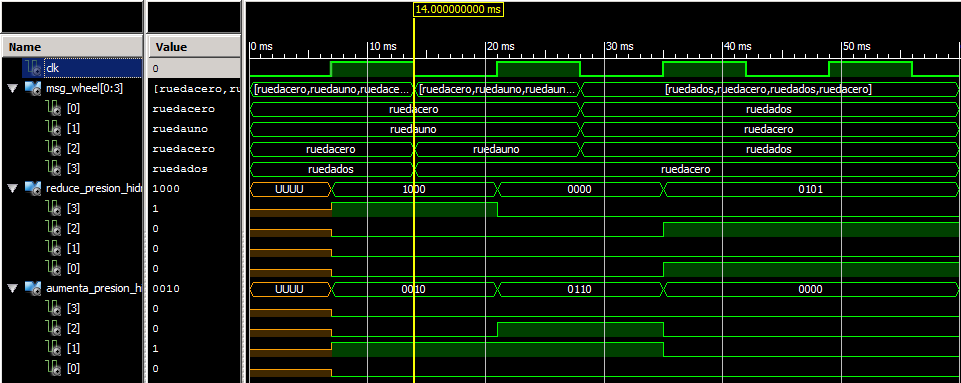
\includegraphics[width=1\textwidth]{img/p4_tb_wheel.png}
  \caption{Resultado obtenido en la simulación de la ECU al probar el control de estabilidad.}
  \label{fig:p4:tb_wheel}
\end{figure}

\clearpage

\section{Práctica 5: Secuencia de Números Binarios Pseudo-Aleatorios.}

\subsection{Enunciado.}

En numerosas aplicaciones es preciso generar números aleatorios para acelerar procesos que simulados en PCs suelen tardar una cantidad de tiempo considerable. Esta aleatoriedad deseada se suele asociar al término ruido blanco, el cual es un tipo de ruido impredicible muy habitual en telecomunicaciones.

Dado que no es habitual que exista de manera nativa una fuente de ruido blanco que permita obtener números puramente aleatorios, en un FPGA se suele recurrir a un registro generador de secuencias binarias pseudo-aleatorias (PRBS, \textit{Pseudo-Random Binary Sequence}). Al contrario que el ruido blanco una PRBS es predicible, dado que se repite cada \emph{m} bits, pero si se trocea en varias partes más pequeñas, parecerá que la sucesión de subsecuencias es realmente aleatoria (obviamente cuanto más grande sea \emph{m}, más aleatoria parecerá).

Una forma fácil de crear una PRBS consiste en hacer uso de un registro de desplazamiento en el que algunos bits realimentan (tras pasar por una XOR o una XNOR) al bit más significativo. La figura \ref{fig:p5:prbs} ilustra esta idea. La salida del sistema es una secuencia denominada PN (\emph{Pseudo-Noise}) o PRN (\emph{Pseudo-Random Noise}) que está constituida por el valor del registro.

\textbf{Atención:} el registro mostrado en la figura \ref{fig:p5:prbs} genera números aleatorios pero no tiene período máximo (sólo para el caso de 4 bits). Para obtener un periodo máximo, habría que crear el registro utilizando puertas XNOR.

\begin{figure}[h]
  \centering
    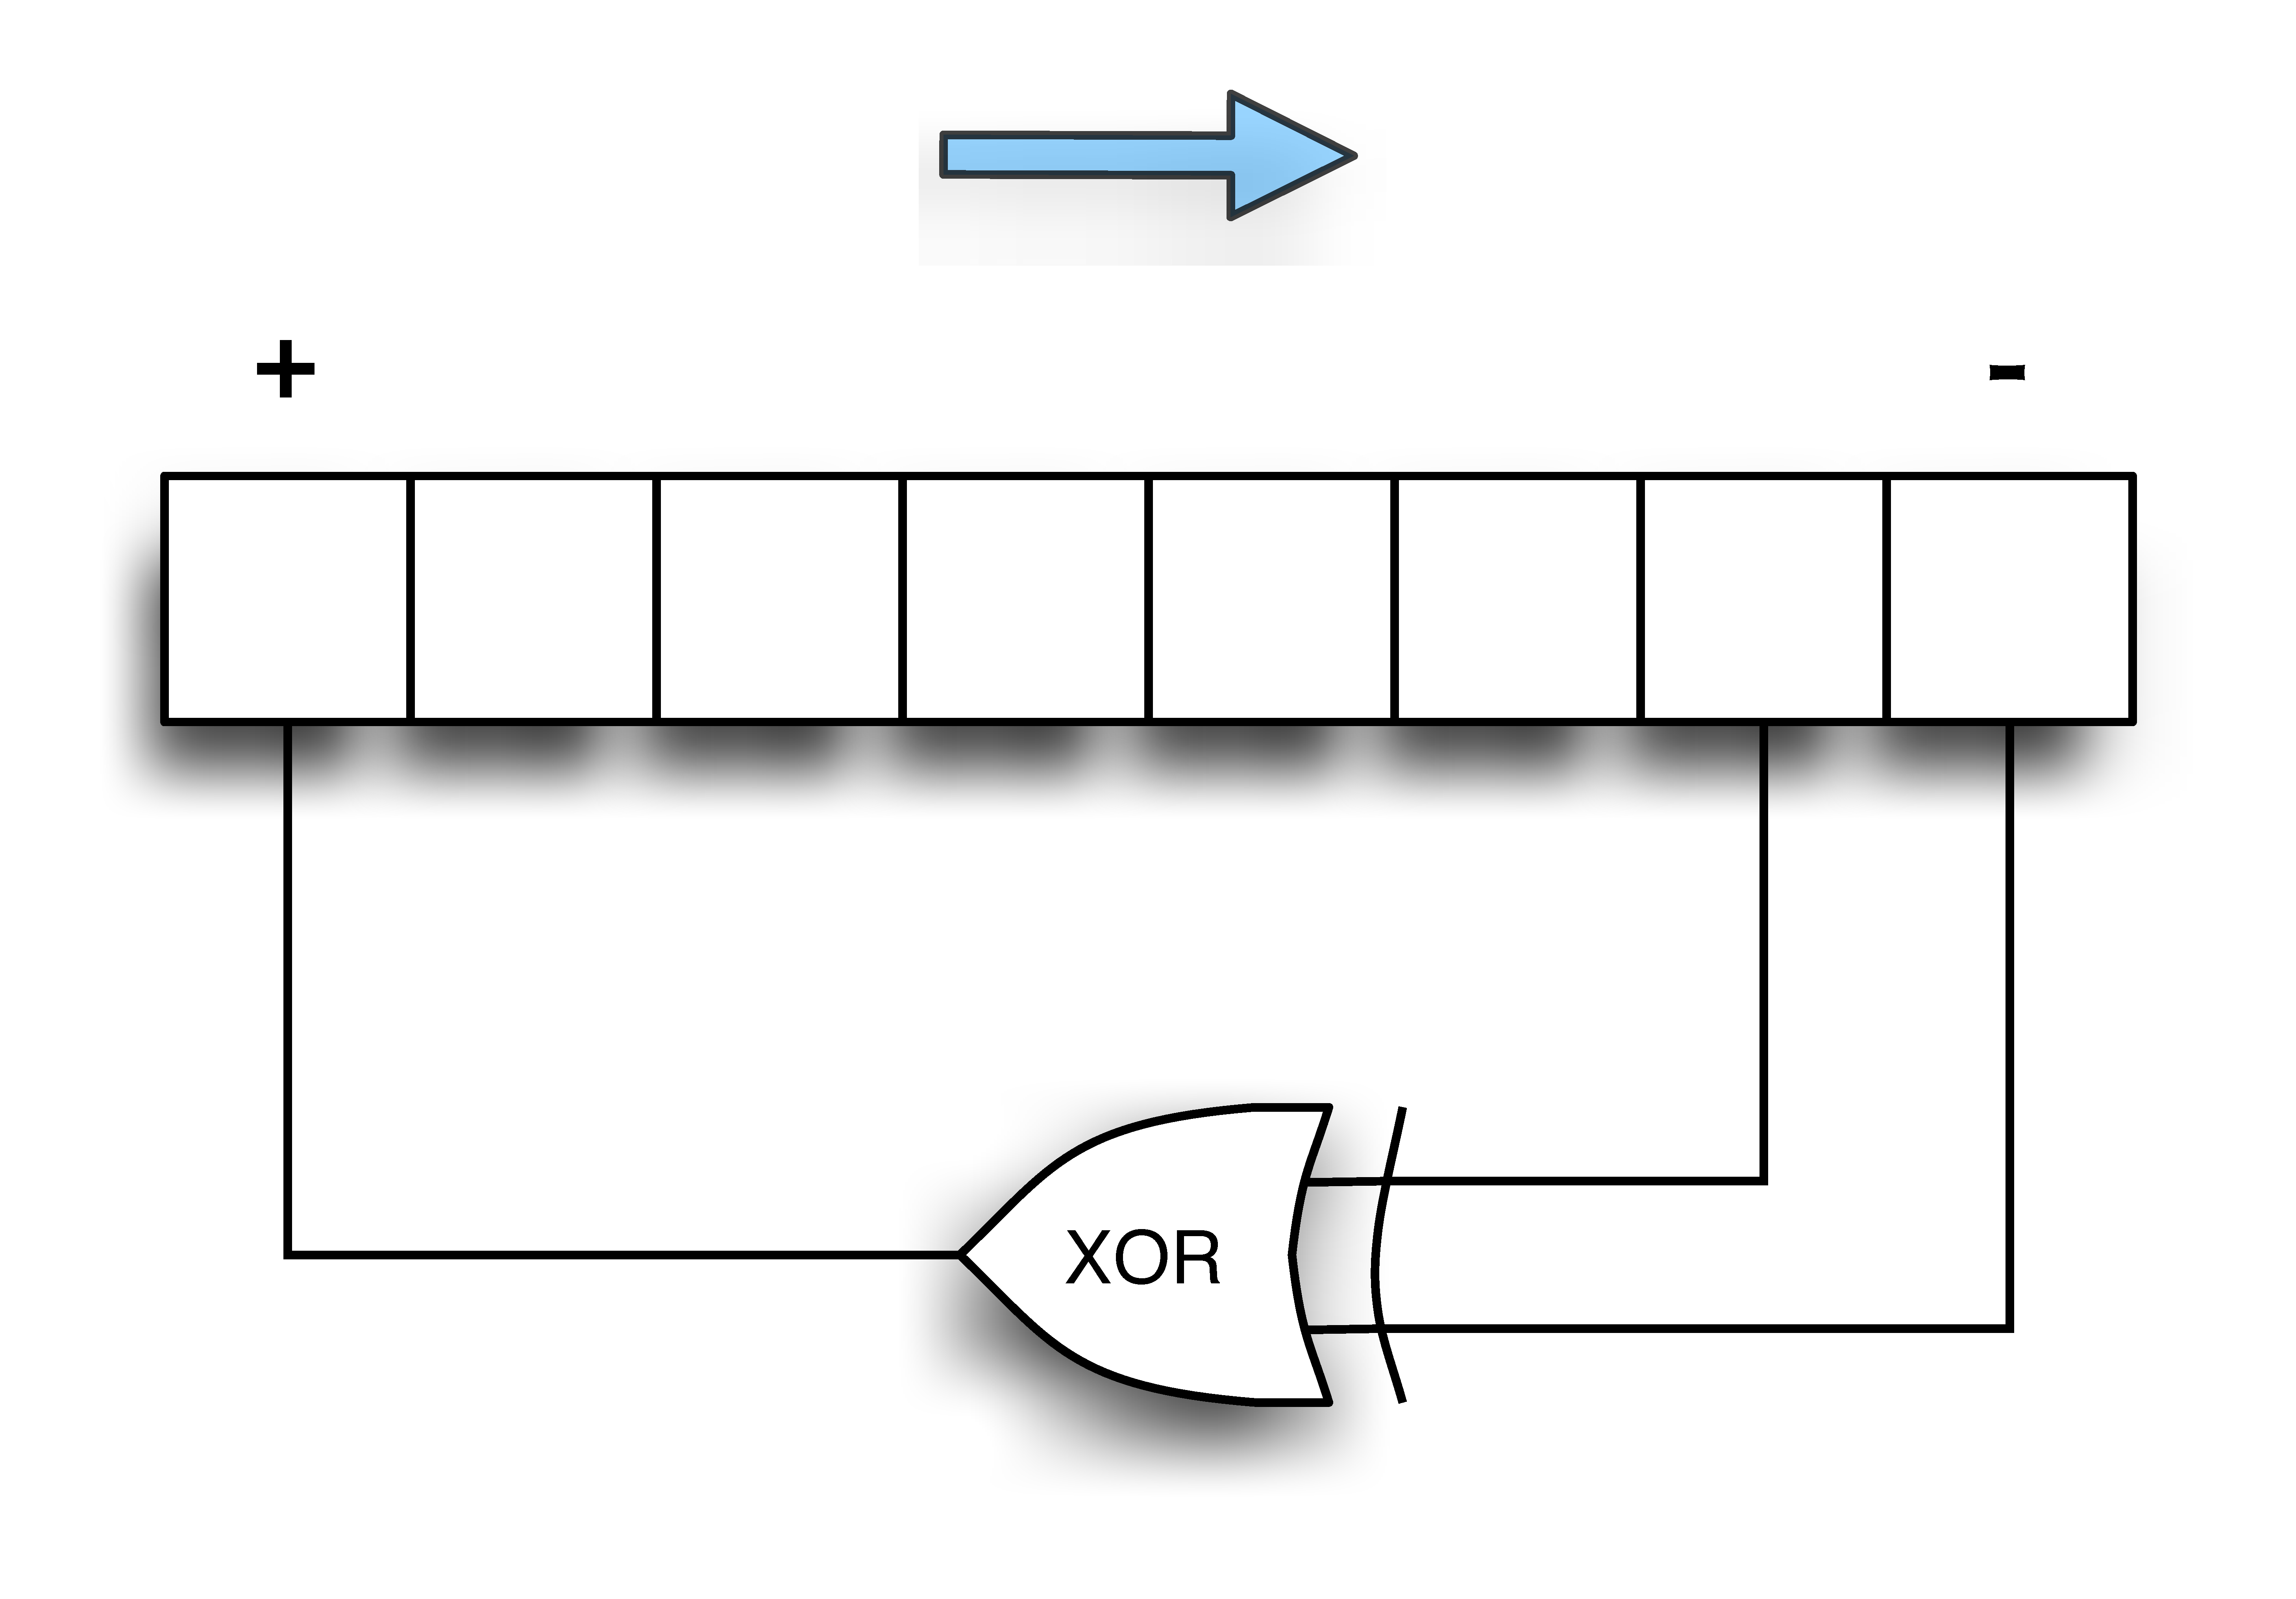
\includegraphics[width=0.3\textwidth]{img/PRBS.pdf}
  \caption{Ejemplo de registro PRBS.}
  \label{fig:p5:prbs}
\end{figure}

Si en lugar de coger el valor de la secuencia se utiliza bit a bit se puede determinar si ésta es pseudo-aleatoria a través de la autocorrelación:

\newtheorem*{corolario}{Lema}
\begin{corolario}
	Dada una secuencia de N bits $x_i$ (con i entre 0 y N-1), la cual posee m unos y N-m ceros, se dirá que es pseudo-aleatoria cuando su función de autocorrelación
	\begin{equation}
		AC(v) = \sum_{i=0}^{N-1} X_i X_{i+v}
	\end{equation}
	tome únicamente dos valores:
	\begin{equation}
		AC(v) = 
		\left\{
			\begin{array}{ll}
				m & \mathnormal{si\ v = 0\ (mod\ N)} \\
				\frac{m*(m-1)}{N-1} & \mathnormal{en\ otro\ caso}
			\end{array}
		\right.
	\end{equation}	
\end{corolario}



\subsection{Apartado A.}

	En este apartado se pide diseñar e implementar la estructura del registro PRBS teniendo en cuenta que se deberá actualizar en cada ciclo de reloj. El comportamiento del PRBS debe seguir el esquema mostrado en la figura \ref{fig:p5:prbs} y debe tener una longitud configurable en tiempo de síntesis a través de una constante.
	
\subsubsection{Implementación.}

	La implementación del PRBS recibe como única entrada una semilla de tipo \emph{BIT\_VECTOR} a partir de la cual se comenzarán a generar las secuencias binarias pseudo-aleatorias. El tamaño de la semilla debe ser el mismo que el del número de bits del registo. Dicho número se indica en la constante \emph{S\_LENGTH} de tipo entero que está definida en un paquete para poder ser usada en la \emph{entity} en la cual se definen las entradas y salidas de la FPGA (véase la figura \ref{cod:p5a:package}). Al estar definida la longitud como una constante permite que si se desea cambiar el tamaño del registro generador de secuencias binarias pseudo-aleatorias sea tan sencillo como cambiar el valor de dicha constante. La salida de la FPGA es una señal de tipo \emph{BIT\_VECTOR} y cuyo número de bits es el indicado en la constante \emph{S\_LENGTH}. En ella se muestra la secuencia binaria pseudo-aleatoria generada en cada ciclo de reloj.
	
	Además de tener como entrada la semilla (\emph{srandom}), y el registro con la salida (\emph{sequence}) se ha añadido la señal de reloj (\emph{CLK}) para simular un PRBS. En la figura \ref{cod:p5a:entity} se puede ver la interfaz usada.
	
\begin{figure}[h]
	\begin{lstlisting}[style=vhdl]
PACKAGE cte IS
	CONSTANT S_LENGTH : INTEGER := 15; -- Le restamos 1 a la longitud que queremos
	--(por ejemplo para longitud 4 hay que poner 3, para longitud 16 poner 15)
end cte;
	\end{lstlisting}
	\caption{Paquete con definición de la constante que especifica el tamaño del registro.}
	\label{cod:p5a:package}
\end{figure}


\begin{figure}[h]
	\begin{lstlisting}[style=vhdl]
entity p5a is
    Port ( CLK      : in  STD_LOGIC;
           srandom  : in  BIT_VECTOR (S_LENGTH downto 0);
           sequence : out BIT_VECTOR (S_LENGTH downto 0)
			 );
end p5a;
	\end{lstlisting}
	\caption{Definición de la interfaz}
	\label{cod:p5a:entity}
\end{figure}

El PRBS dentro de la FPGA se simula como un proceso cuya lista de sensibilidad es la señal de entrada de reloj y la semilla con la que se inicializa el registro. Dicho proceso realiza las operaciones en el flanco positivo de la señal de reloj (que se consigue usando la función \emph{rising\_edge(CLK)}) Dentro del proceso existe una variable del tipo \emph{BIT\_VECTOR} cuyo tamaño está especificado en la constante \emph{S\_LENGTH} en la que se realizan las operaciones XOR y de desplazamiento. Una vez se tiene calculada la nueva secuencia se copia el valor en la señal de salida. La implementación del proceso se puede ver en la imagen \ref{cod:p5a:process}.
	
\begin{figure}[h]
	\begin{lstlisting}[style=vhdl]
process (CLK, srandom)
	VARIABLE tmp : BIT_VECTOR (S_LENGTH downto 0);
begin
	-- Para que la primera vez se inicalice la secuencia con la semilla
	if (srandom'EVENT) then
		tmp := srandom;
	end if;
	
	if (rising_edge(CLK)) then
		tmp := (tmp(0) XOR tmp(1)) & tmp(S_LENGTH downto 1);
		-- se copia el valor temporal a la secuencia
		sequence <= tmp;
	end if;
end process;
	\end{lstlisting}
	\caption{Implementación del PRBS para el apartado A.}
	\label{cod:p5a:process}
\end{figure}

\subsubsection{Test.}

	Para comprobar el funcionamiento del PRBS se ha desarrollado un \emph{Test Bench}. El test se ha realizado para un registro de 4 bits y para otro de 16 bits.

	\vspace{0.5cm} % Para dejar un espacio	
	\textbf{Registro de 4 bits.}

	El registro se ha inicializado con la semilla \emph{0110}. En la figura \ref{fig:p5a:tb_4bits} se puede comprobar como a partir de los 1650 nanosegundos se cumplen las 15 combinaciones posibles y la secuencia de bits se vuelve a repetir. Hay que tener en cuenta que la combinación 0000 haría que el PRBS siempre daría el mismo resultado porque la operación XOR siempre devolvería un valor de 0.
	
\begin{figure}[h]
  \centering
    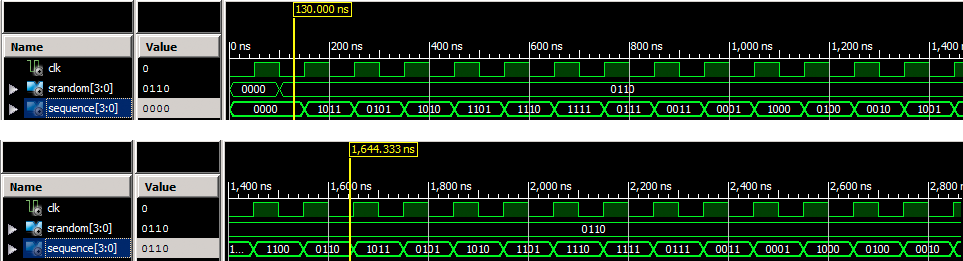
\includegraphics[width=1\textwidth]{img/p5a_tb_4bits.png}
  \caption{Resultados obtenido con un PRBS de 4 bits.}
  \label{fig:p5a:tb_4bits}
\end{figure}

	\vspace{0.5cm} % Para dejar un espacio	
	\textbf{Registro de 16 bits.}
	
	La semilla con la que se empieza a genera los números pseudo-aleatorios tiene el valor de \emph{0110011010100110}. En la figura \ref{fig:p5a:tb_16bits} se puede comprobar el inicio del comportamiento esperado. No se muestran todas las posibles combinaciones por el gran número de combinaciones que puede dar.

\begin{figure}[h]
  \centering
    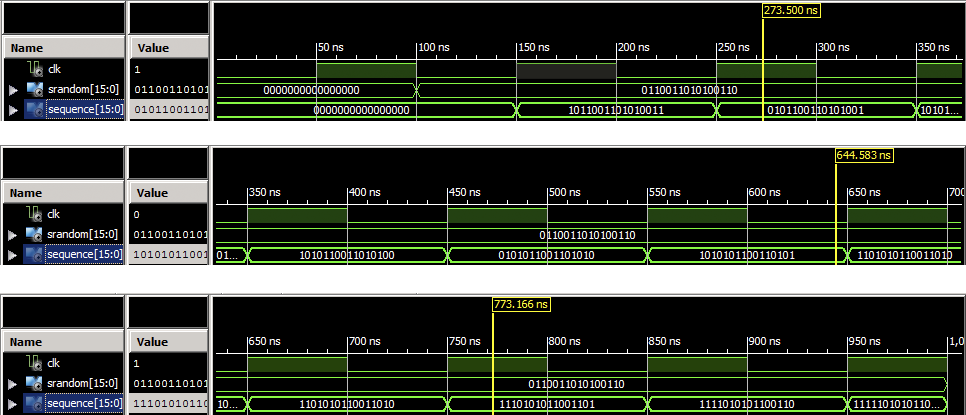
\includegraphics[width=1\textwidth]{img/p5a_tb_16bits.png}
  \caption{Resultados obtenido con un PRBS de 16 bits.}
  \label{fig:p5a:tb_16bits}
\end{figure}

\subsection{Apartado B.}

	En este apartado se pide diseñar e implementar un registro PRBS optimizado para tener ciclo máximo para secuencias de 40 bits.
	
	A mayores se pide añadir una función que calcule el valor de la autocorrelación para subsecuencias de 4 bits (\textbf{luego en la fórmula de la autocorrelación, v es igual a 4}) sobre la sequencia global de 40 bits. La salida de la autocorrelación debe enlazarse con una señal para poder mostrar el resultado al simular.

\subsubsection{Implementación.}

	Para implementar un registro PRBS optimizado para tener ciclo máximo para secuencias de 40 bits se han utilizado los datos de la ``\textit{Tabla para creación de registros PRBS de n bits con período máximo}'' que aparece en el boletín de la práctica. EL fragmento de la tabla que no interesa se puede ver en la tabla \ref{tab:p5b:PRBS_max}.

\begin{table}
	\begin{center}
		\begin{tabular}{|c|c|}
\hline
\textbf{N} & \textbf{XNOR sobre los bits} \\ \hline

\multicolumn{2}{c}{\vdots} \\ \hline
39 & 39, 35\\ \hline
\textbf{40} & \textbf{40, 38, 21, 19} \\ \hline
41 & 41, 38\\ \hline
\multicolumn{2}{c}{\vdots} \\ 
		\end{tabular}
		\caption{Tabla para la creación de registros PRBS de 39, 40 y 41 bits con periodo máximo.}
		\label{tab:p5b:PRBS_max}
	\end{center}
\end{table}

El funcionamiento del PRBS implementado en el apartado B consiste en:
\begin{enumerate}
	\item Calcular el valor de la operación XNOR de los bits 40, 38, 21 y 19 del registro.
	\item Desplazar todos los bits del registro una posición a la derecha.
	\item Añadir el bit resultado de la operación XNOR calculado en el paso 1 a la izquierda del registro.
\end{enumerate}
A mayores también hay que calcular la autocorrelación de la secuencia de bits calculada en los pasos anteriores. En la figura \ref{cod:p5b:autocorrelacion} se puede consultar la implementación de la función que calcula la autocorrelación mientras que el proceso que ejecuta la implementación del PRBS del apartado B se puede ver en la figura \ref{cod:p5b:process}.

\begin{figure}[h]
	\begin{lstlisting}[style=vhdl]
function autocorrelation (v: INTEGER; sequence: BIT_VECTOR (S_LENGTH downto 0)) return integer is
	variable r: integer := 0;
begin
	-- se suma si los dos bits cumplen la condicion de autocorrelacion
	for i in 0 to S_LENGTH -v loop
		if sequence(i) = '1' and sequence(i+v) = '1' then
			r := r + 1;
		end if;
	end loop;
	
	return r;
end autocorrelation;
	\end{lstlisting}
	\caption{Función para calcular la autocorrelación de una secuencia de bits.}
	\label{cod:p5b:autocorrelacion}
\end{figure}

\begin{figure}[h]
	\begin{lstlisting}[style=vhdl]
process (CLK, srandom)
	VARIABLE tmp : BIT_VECTOR (S_LENGTH downto 0);
begin
	-- Para que la primera vez se inicalice la secuencia con la semilla
	if (srandom'EVENT) then
		tmp := srandom;
	end if;
	
	if (rising_edge(CLK)) then
		tmp := (tmp(39) XNOR tmp(37) XNOR tmp(20) XNOR tmp(18)) & tmp(S_LENGTH downto 1);
		-- se copia el valor temporal a la secuencia
		sequence <= tmp;
		-- se calcula la autocorrelacio
		value <= autocorrelation(4, tmp);
	end if;
end process;
	\end{lstlisting}
	\caption{Implementación del PRBS para el apartado B.}
	\label{cod:p5b:process}
\end{figure}

\subsubsection{Test.}

	Para ver el comportamiento del PRBS se ha desarrollado un \emph{Test Bench}. La semilla utilizada para realizar la prueba ha sido: \emph{1110110010110010101101001010000110101010}.
	En la figura \ref{fig:p5b:tb} se muestra la vista de como va evolucionando el valor que se corresponde con la autocorrelación.

\begin{figure}[h]
  \centering
    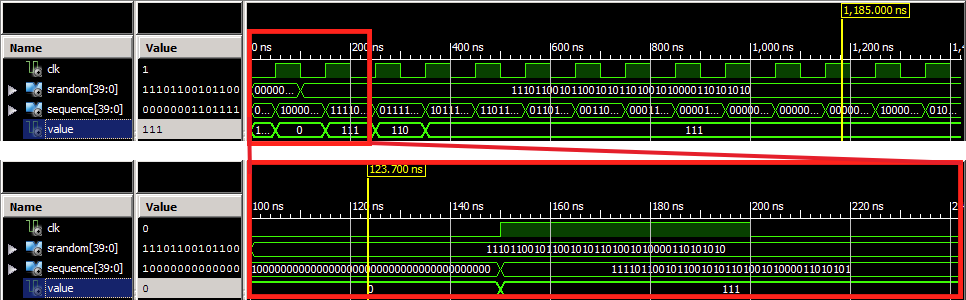
\includegraphics[width=1\textwidth]{img/p5b_tb.png}
  \caption{Simulación realizada con el PRBS del apartado B.}
  \label{fig:p5b:tb}
\end{figure}

\section{Práctica 6: Sistema de adelantamiento inteligente.}

\subsection{Enunciado.}

	En esta práctica, vamos a suponer que poseemos un vehículo que tiene instalado un sistema de cámaras conectadas a una FPGA. Este sistema entra en funcionamiento sólo cuando el conductor utiliza los intermitentes al señalizar un adelantamiento, evitando así su uso en casos en los que se precisa realizar maniobras rápidas para evitar colisiones.
	
	Una de las cámaras estaría situada bajo un retrovisor y permitiría saber si existen o no vehículos en el carril adyacente, bien sea porque se aproximan a nuestro vehículo por dicho carril, o bien porque circulan por el ángulo muerto. En el caso de que existiese posibilidad de colisión, el sistema prevendría al conductor emitiendo un pitido.
	
	Por otro lado, una segunda cámara estaría colocada en la parte frontal del vehículo y serviría para detectar si las líneas del carril son continuas o discontinuas. Si el conductor intenta realizar el adelantamiento en una zona con líneas continuas, el sistemas intentará evitar la maniobra, indicando al sistema de control central (por ejemplo, a través de la ECM o la ECU) que debe incrementarse la resistencia de la dirección.

	Para modelar este sistema de control de adelantamientos se pide diseñar el diagrama de estados de la lógica de control del sistema. Debe tenerse en cuenta que va a haber una señal inicial INTERMITENTE\_ENCENDIDO que indica que va a realizar un adelantamiento. Además, se considerará como estado inicial el estado OBTENER\_IMAGENES y la información suministrada por cada cámara se representará por un único bit (carril adyacente libre/ocupado y líneas continuas/discontinuas). Cada estado estará asociado a una variable binaria distinta que indicará si se lleva a cabo la acción o no.

\subsection{Implementación.}
	Para empezar con la implementación primero tenemos que tener la máquina de estados en la que puede estar el sistema de control. Los posibles estados se muestran en la tabla \ref{tab:p6:estados}
	
\begin{table}
	\begin{center}
		\begin{tabular}{|c|c|}
\hline
\textbf{Código} & \textbf{Estado} \\ \hline
\hline
obtener imágenes & Estado inicial al que se accede al activar el intermitente.\\ \hline
$q_0$ & Se puede realizar el adelantamiento\\ \hline
$q_1$ & Hay una línea continua (endurecer dirección)\\ \hline
$q_2$ & Carril adyacente ocupado (emitir pitido)\\ \hline
$q_3$ & Carril adyacente ocupado y línea continua (endurecer dirección y emitir pitido)\\ \hline
intermitente apagado & Estado final al que se accede cuando se apaga el intermitente\\ \hline
		\end{tabular}
		\caption{Tabla con los posibles estados.}
		\label{tab:p6:estados}
	\end{center}
\end{table}

	Lo siguiente es tener las tener las transiciones entre estados tal y como se muestra la de la figura \ref{fig:p6:estados}.

\begin{figure}[h]
  \centering
    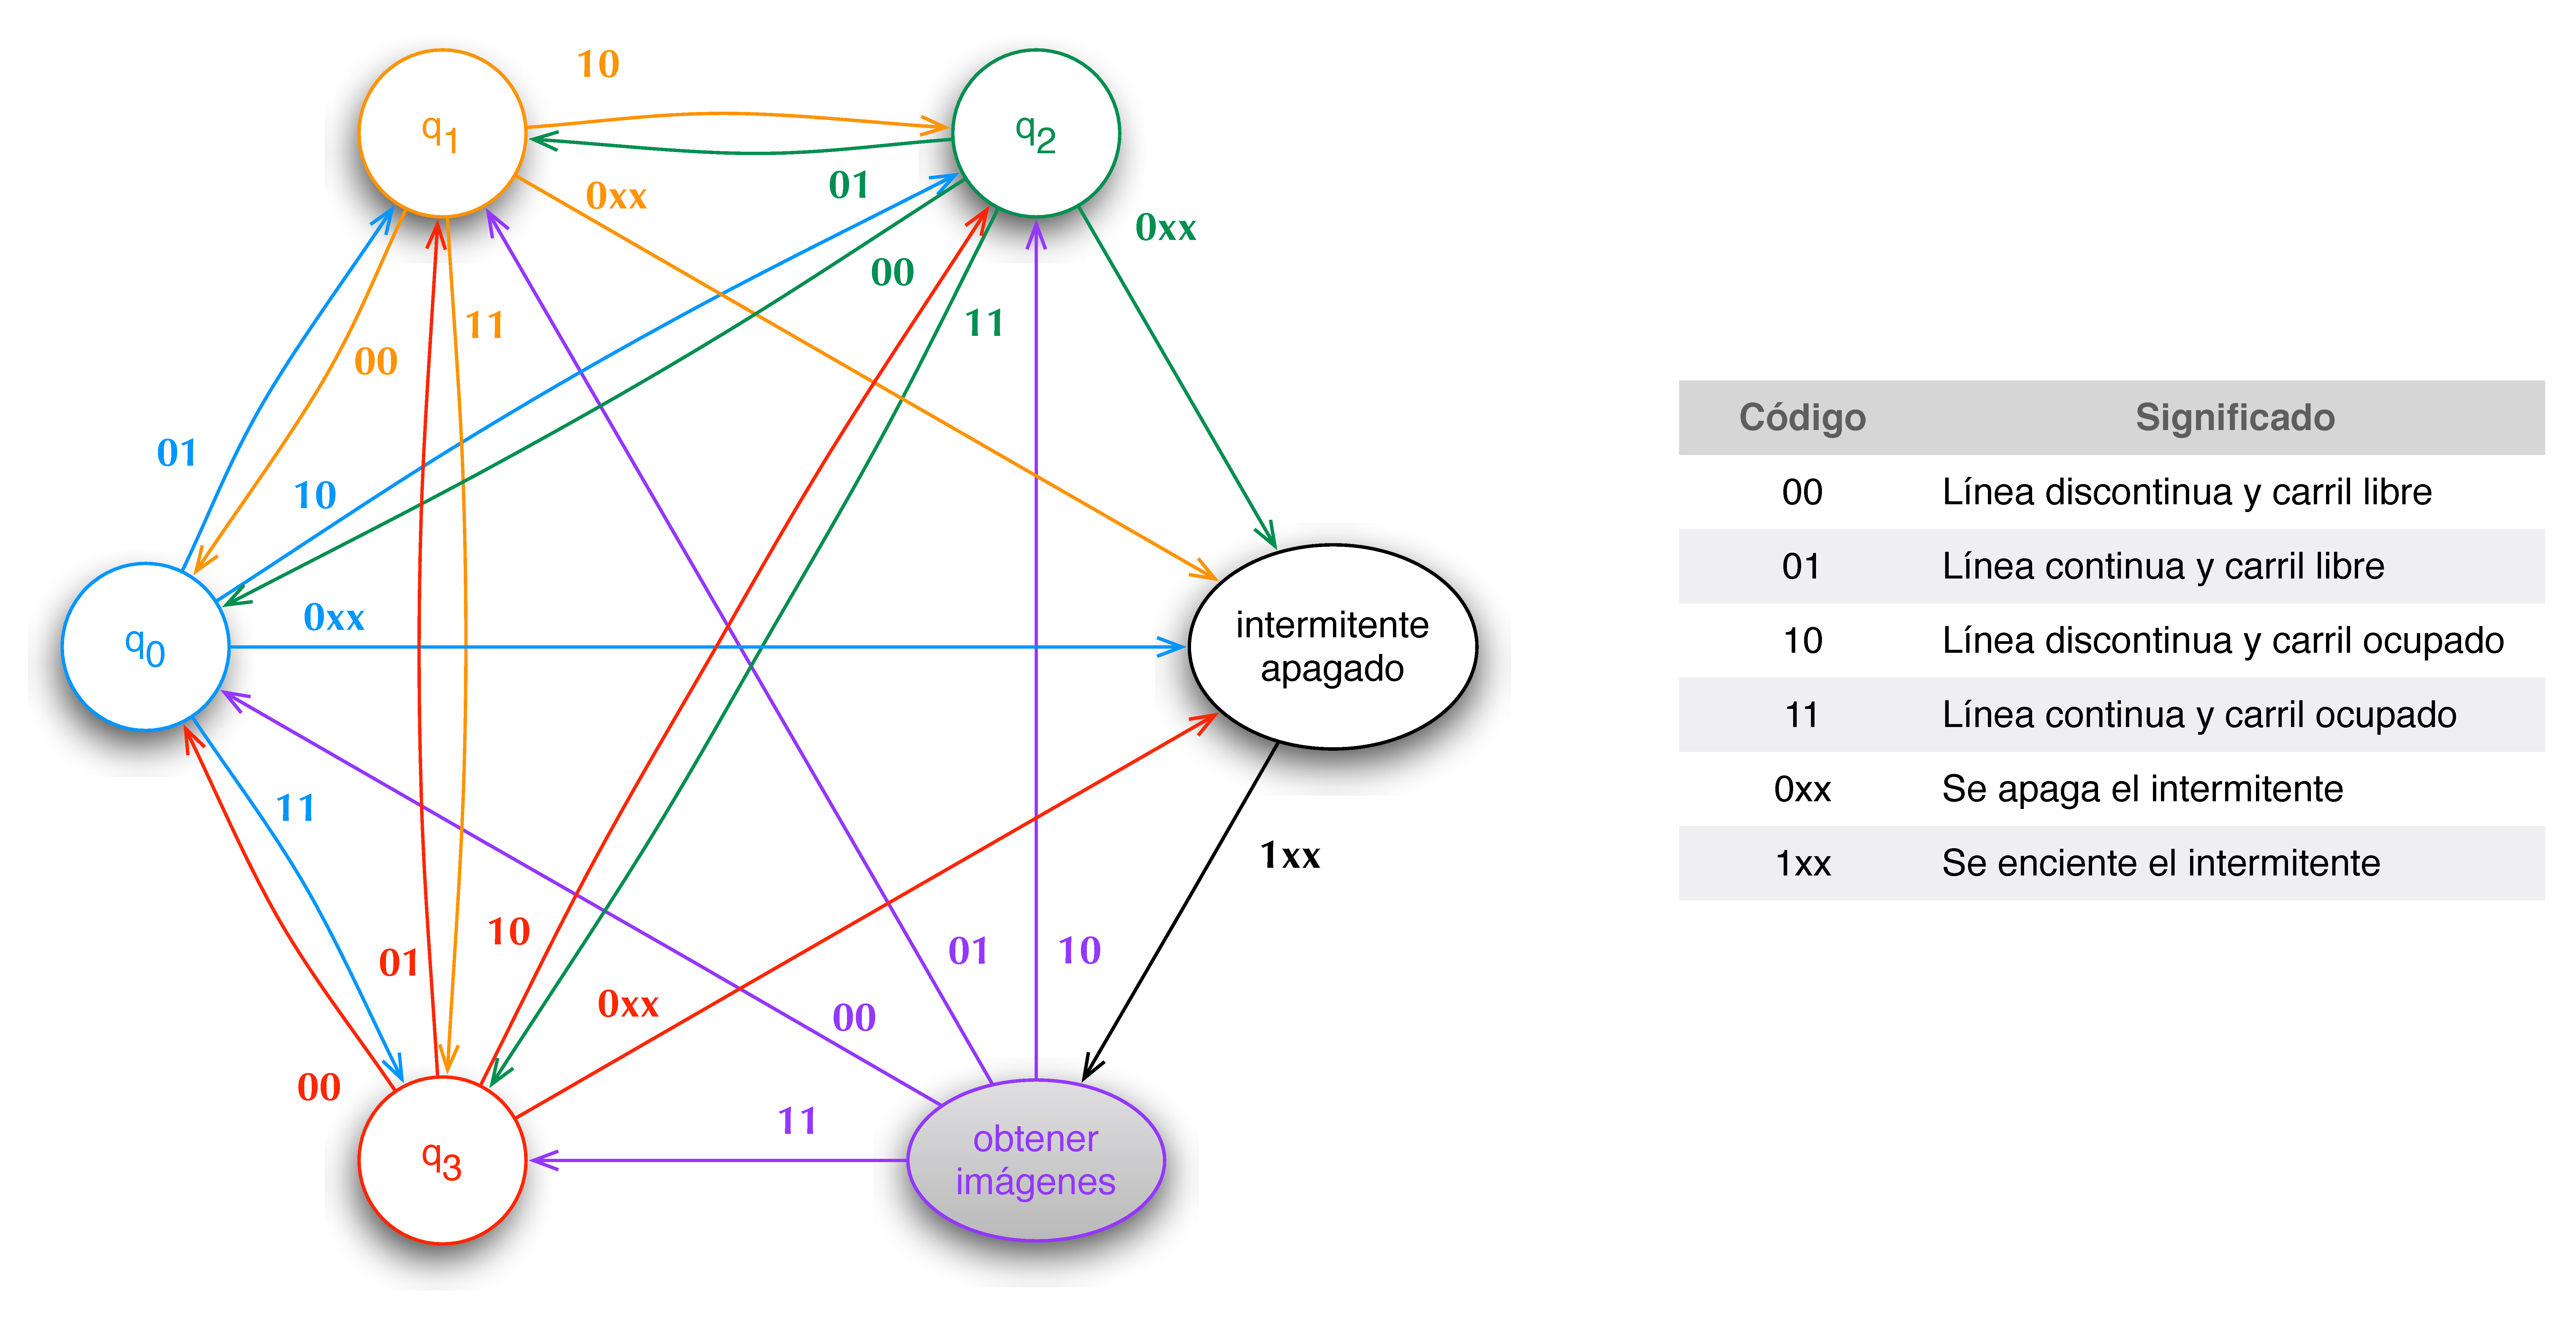
\includegraphics[width=1\textwidth]{img/maquina_estados.pdf}
  \caption{Máquina de estados.}
  \label{fig:p6:estados}
\end{figure}

	Ahora llega el momento de identificar cuales van a ser las entradas y salidas de la FPGA para la implementación del sistema inteligente. Para ello tendremos dos entradas, una que indica si el carril adyacente está ocupado (\emph{way}) y la otra que indica si hay línea continua (\emph{line}) mientras que las dos salidas que tenemos tienen la función de emitir un pitido (\emph{sound}) o endurecer la dirección (\emph{stiffen}). A mayores lo sincronizaremos todo con una señal de reloj (\emph{CLK}). En la figura \ref{cod:p6:entity} podemos ver el \emph{entity} que muestra las salidas y las entradas al sistema.
	
\begin{figure}[h]
	\begin{lstlisting}[style=vhdl]
entity p6 is
    Port ( CLK       : in  STD_LOGIC;
			  indicator : in  BIT; -- 1 -> intermitente encendido
           way       : in  BIT; -- 1 -> camino ocupado
           line      : in  BIT; -- 1 -> linea continua
			  
           sound   : out  BIT; -- 1 -> emitir pitido
           stiffen : out  BIT  -- 1 -> endurecer direccio
			 );
end p6;
	\end{lstlisting}
	\caption{Definición de la interfaz.}
	\label{cod:p6:entity}
\end{figure}

La maquina de estados se implementa usando dos procesos. Uno encargado de la lógica de control y otro encargado de actualizar el estado. El proceso encargado de la lógica de control (figura \ref{cod:p6:control_process}) tiene como lista de sensibilidad las señales de estado actual(\emph{current\_state}), indicador de carril adyacente ocupado (\emph{way}) y el indicador  de línea ocupada (\emph{line}). El proceso encargado de actualizar el estado actual (figura \ref{cod:p6:control_update}) tiene como lista sensibilidad la señal de reloj (\emph{CLK}) y la señal que indica si el intermitente está encendido (\emph{indicator}).

Los posibles estados en los que se puede encontrar la máquina de estados están definidos como un tipo enumerado que tiene el nombre \emph{state} y se ha definido de la siguiente manera:
\begin{lstlisting}[style=vhdl]
	type state is (INDICATOR_OFF, GET_PICTURES, Q0, Q1, Q2, Q3);
\end{lstlisting}

También se han declarado dos señales de tipo \emph{state} para almacenar el valor del estado actual (\emph{current\_state}) y del estado siguiente (\emph{next\_state}):
\begin{lstlisting}[style=vhdl]
	signal current_state: state;
	signal next_state   : state;
\end{lstlisting}

\begin{figure}[h]
	\begin{lstlisting}[style=vhdl]
process (current_state, way, line)
	variable aux : BIT_VECTOR(1 downto 0);
begin
	aux := way & line;
	case current_state is
		when INDICATOR_OFF =>
			sound <= '0';
			stiffen <= '0';
			next_state <= INDICATOR_OFF;
		when GET_PICTURES =>
			sound <= '0';
			stiffen <= '0';
			next_state <= get_next_state(aux);
		when Q0 =>
			sound <= '0';
			stiffen <= '0';
			next_state <= get_next_state(aux);
		when Q1 =>
			sound <= '0';
			stiffen <= '1';
			next_state <= get_next_state(aux);
		when Q2 =>
			sound <= '1';
			stiffen <= '0';
			next_state <= get_next_state(aux);
		when Q3 =>
			sound <= '1';
			stiffen <= '1';
			next_state <= get_next_state(aux);
		when others =>
			sound <= '0';
			stiffen <= '0';
			next_state <= INDICATOR_OFF;
	end case;
end process;
	\end{lstlisting}
	\caption{Implementación del proceso encargado de la lógica de control. La implementación de la función \emph{get\_next\_state} se muestra en la figura \ref{cod:p6:get_next_state}.}
	\label{cod:p6:control_process}
\end{figure}
	
\begin{figure}[h]
	\begin{lstlisting}[style=vhdl]	
process (CLK, indicator)
begin
	if (indicator'EVENT) then
		if (indicator = '1') then
			current_state <= GET_PICTURES;
		else
			current_state <= INDICATOR_OFF;
		end if;
	elsif (rising_edge(CLK)) then
		current_state <= next_state;
	end if;
end process;
	\end{lstlisting}
	\caption{Implementación del proceso encargado de actualizar el estado.}
	\label{cod:p6:control_update}
\end{figure}	

\begin{figure}[h]
	\begin{lstlisting}[style=vhdl]	
-- aux(0) = linea continua?
-- aux(1) = posible colision?
function get_next_state(aux : BIT_VECTOR(1 downto 0)) return state is
  variable aux_state: state;
begin
	case aux is
		when "00" => aux_state := Q0;
		when "01" => aux_state := Q1;
		when "10" => aux_state := Q2;
		when "11" => aux_state := Q3;
	end case;
	return aux_state;
end get_next_state;
	\end{lstlisting}
	\caption{Función que dependiendo de las dos señales que existen de entrada indican cual sería el siguiente estado (siempre y cuando no se apague el intermitente).}
	\label{cod:p6:get_next_state}
\end{figure}	

\subsection{Test.}

	Para poder comprobar que la máquina de estados funciona correctamente se ha desarrollado un \emph{Test Bench}. La comprobación se ha realizado siguiendo los pasos de una posible simulación de un viaje que se muestran a continuación:
	
\begin{enumerate}
	\item Encendemos el intermitente porque queremos comenzar un adelantamiento.
	\item La cámara detecta que hay una línea continua.
	\item Ahora también se detecta un coche por el carril adyacente
	\item Se libera el carril adyacente y comienza una zona con  línea discontinua.
	\item Apagamos el intermitente.
	\item Encendemos el intermitente para adelantar.
	\item La cámara detecta que hay un coche en el carril adyacente.
	\item Apagamos el intermitente.
	\item Como queremos adelantar lo indicamos encendiendo el intermitente.
	\item Hay una línea continua y un coche en el carril adyacente.
	\item Estamos en una zona sin coches en el carril adyacente y con línea discontinua y podemos efectuar el adelantamiento.
	\item Como hemos realizado el adelantamiento apagamos el intermitente.
\end{enumerate}

\section{Práctica 7: Segmentación de imágenes.}

\subsection{Enunciado.}

	En esta práctica vamos a implementar en VHDL un sencillo segmentador de imágenes que nos permita identificar determinados patrones en base a valores RGB. Para ello supongamos que nuestro objetivo es realizar un sistema de detección de incendios forestales basado en FPGAs que procesan la información procedente de cámaras que suministran imágenes periódicamente. Estos dispositivos de monitorización de incendios estarán ubicados en dos tipos de localizaciones: en postes/árboles diseminados por el bosque y en UAVs (\textit{Unmanned Aerial Vehicles}) que realizan recorridos sobre las zonas de monte más inaccesibles.
	
	Los dispositivos situados en los postes/árboles deben detectar la presencia de fuego a distancias relativamente cercanas, mientras que los UAVs han de ser capaces de localizar humaredas sobre las superficies arboladas.

\subsection{Primer apartado.}

	Diseñar e implementar en VHDL el segmentador de imágenes haciendo uso de un único proceso. Este proceso será el encargado de tratar los valores del fichero de entrada e irá escribiendo el resultado en un fichero con el mismo formato que el de entrada.
	
	Hay que verificar que el resultado es el deseado  visualizando la imagen resultante en Matlab.

\subsubsection{Implementación.}
	En esta práctica la la entrada/salida se realiza mediante ficheros que contiene el valor de los pixels de una imagen y se escribe en otro fichero con el valor de los pixels resultantes del filtrado.

	Los ficheros empleados son ficheros de texto. Están estructurados en tras partes. Una parte para cada capa de color de la imagen (capa R, capa G, capa B). A mayores también se decide crear un fichero de una capa que contiene valores binarios en el que se puede ver el perfil detectado mediante la segmentación.
	
	Para empezar con la implementación lo primero que se realizó fue la declaración de algunos tipos de datos y algunas constantes (vease figura \ref{cod:p7a:tiposYctes}). Los tipos que se declararon fueron:
\begin{itemize}
	\item \emph{minimax}: Es un array que contiene dos valores donde la primera posición es para indicar un mínimo mientras que la otra es para especificar un máximo. Esto sirve para que tengamos que cumplir un mínimo y máximo para cada componente.
	\item \emph{components}: Es un enumerado para especificar las componentes del espacio de color RGB.
	\item \emph{image}: Es un array bidimensional en el que se puede almacenar una componente de color de la imagen. 
\end{itemize}
	Las constantes que se han declarado son para hacer más fácil cualquier mínimo cambio que se requiera. Por esta razón se declararon las variables:
\begin{itemize}
	\item \emph{height}: Especifica el largo de la imagen.
	\item \emph{width}: Especifica el ancho de la imagen.
	\item \emph{t\_red}: Indica los valores de color rojo entre los que puede estar el objeto que se quiere identificar.
	\item \emph{t\_green}: Indica los valores de color verde entre los que puede estar el objeto que se quiere identificar.
	\item \emph{t\_blue}: Indica los valores de color azul entre los que puede estar el objeto que se quiere identificar.
	\item \emph{input\_file}: Es la ruta al fichero que tiene la imagen de entrada.
	\item \emph{output\_rgb}: Es la ruta al archivo que contendrá la imagen segmentada.
	\item \emph{output\_bin}: Es la ruta de la imagen que tendrá los valores binarios de la umbralización.
	\item \emph{background}: Es el color que se quiere dar de fondo para la imagen que tendrá el objeto segmentado.
\end{itemize}

\begin{figure}[h]
	\begin{lstlisting}[style=vhdl]	
	type minimax is array (0 to 1) of integer; -- 0 min, 1 max  
	
	type components is (red, green, blue);
	
	constant height: integer := 480; -- largo
	constant width : integer := 360; -- ancho
	
	type image is array (1 to height, 1 to width) of integer; -- tipo para guardar una imagen

	constant t_red   : minimax := (210, 255); -- valores minimo y maximo entre los que tiene que estar la componente roja
	constant t_green : minimax := (100, 255); -- valores minimo y maximo entre los que tiene que estar la componente verde
	constant t_blue  : minimax := (0, 210); -- valores minimo y maximo entre los que tiene que estar  la componente azul
	
	file input_file : text open read_mode  is "lume.imfpga";  -- ficheros de entrada y salida
	file output_rgb : text open write_mode is "lume_salida.imfpga";
	file output_bin : text open write_mode is "lume_binaria.imfpga";
	
	constant background: integer := 255; -- fondo que se pone en la imagen rgb
	\end{lstlisting}
	\caption{Constantes y tipos de datos declarados en el primer apartado de la séptima práctica.}
	\label{cod:p7a:tiposYctes}
\end{figure}	

	El único proceso que se podía identificar en esta parte de la práctica se ha creado sin lista de sensibilidad una vez de inicio a fin y se queda parado porque al final hay un \emph{wait}. El flujo que realiza dicho proceso es:
\begin{enumerate}
	\item Leer la imagen de entrada.
	\begin{enumerate}
		\item Leer la componente roja de la imagen.
		\item Leer la componente verde de la imagen.
		\item Leer la componente azul de la imagen.
	\end{enumerate}
	\item Crear la imagen binaria al realizar la umbralización de la imagen leída.
	\item Guardar la imagen binaria de la umbralización.
	\item Guardar la imagen segmentada.
	\begin{enumerate}
		\item Guardar la componente roja de la imagen.
		\item Guardar la componente verde de la imagen.
		\item Guardar la componente azul de la imagen.
	\end{enumerate}
\end{enumerate}

	
\subsubsection{Test.}

	Para poder probar el código una de las cosas que se necesitaba era la de poder leer la imagen binaria que se crea. Para ello se ha creado una función a la cual se le pasa el archivo de salida generado por la FPGA y el tamaño de la imagen original y esta devuelve la imagen del fichero, tanto si como si tiene todas las componentes de color o solo tiene una componente. Esa función se puede ver en la imagen \ref{cod:p7a:read_out_FPGA}.
	
\begin{figure}[h]
	\begin{lstlisting}[style=matlab]	
%% La funcion lee la salida que se ha producido en la fpga.
%  La funcion es capaz de saber si el archivo que se le pasa se corresponde
%  con una componente de color o son varias
% Parametros
%      im_bin       : ruta del archivo de salida de la fpga
%      sizeOriginal : tamano de la imagen original
function [outImage] = read_out_FPGA(im_bin, sizeOriginal)
%% Comprobar el numero de parametros que se pasan a la funcion
    if (nargin ~= 2)
        error('read_out_FPGA: solo admite dos parametros');
    end

%% Se lee el fichero que solo contine caracteres
    try
        fid = fopen(im_bin);
        temp = textscan(fid, '%d');
        fclose(fid);
    catch
        error('read_out_FPGA: No se ha podido acceder al archivo');
    end
    
%% se intenta pasar el archivo a una imagen (comprueba si es para una componente o para varias)
    switch size(sizeOriginal, 2)
        case 2
            if (size(temp{1}, 1) == sizeOriginal(1) * sizeOriginal(2))
                outImage = uint8(reshape(temp{1}, sizeOriginal(1), sizeOriginal(2) ));
            else
                sprintf('El tamano tenia que ser %d pero en cambio es %d\n', sizeOriginal(1) * sizeOriginal(2),size(temp{1}, 1));
                error('read_out_FPGA: El archivo no se ajusta al tamano indicado.'),
            end
        case 3
            if (size(temp{1}, 1) == sizeOriginal(1) * sizeOriginal(2))
                outImage = uint8(reshape(temp{1}, sizeOriginal(1), sizeOriginal(2)));
            elseif (size(temp{1}, 1) == sizeOriginal(1) * sizeOriginal(2)*sizeOriginal(3))
                outImage = uint8(reshape(temp{1}, sizeOriginal(1), sizeOriginal(2), sizeOriginal(3) ));
            else
               sprintf('El tamano tenia que ser %d o %d pero en cambio es %d\n', sizeOriginal(1) * sizeOriginal(2), sizeOriginal(1) * sizeOriginal(2)*sizeOriginal(3),size(temp{1}, 1));
               error('read_out_FPGA: El archivo no se ajusta al tamano indicado!');
            end
        otherwise
            error('read_out_FPGA: El tamano pasado no se corresponde con una imagen');
    end

end
	\end{lstlisting}
	\caption{Función \emph{read\_out\_FPGA.m} hecha en matlab para la lectura de la salida de la FPGA.}
	\label{cod:p7a:read_out_FPGA}
\end{figure}	

	Para facilitar la comprobación de los resultados se ha generado un script en el que se muestran cuatro imágenes:
\begin{enumerate}
	\item La imagen original.
	\item La imagen segmentada.
	\item La imagen binaria.
	\item La imagen segmentada mostrando el fondo en blanco y negro
\footnote{Esta imagen está creada en matlab a partir de la imagen original y la imagen binaria devuelta por la FPGA.}.
\end{enumerate}
	El script se puede consultar en la imagen \ref{cod:p7a:show_output_FPGA}.

\begin{figure}[h]
	\begin{lstlisting}[style=matlab]	
close all;
clear all;
clc;

%% Se cargan los archivos
fire = true;
if (fire)
    inImage = 'lume.png';
    outRGB  = 'lume_salida.imfpga';
    outBIN  = 'lume_binaria.imfpga';
else
    inImage = 'fume.jpg';
    outRGB  = 'fume_salida.imfpga';
    outBIN  = 'fume_binaria.imfpga';
end

%% Se procede a recoger las imagenes
try
    inImage = imread(inImage);
    outRGB  = read_out_FPGA(outRGB, size(inImage));
    outBIN  = read_out_FPGA(outBIN, size(inImage));
catch
   error('Fallo al leer las imagenes de salida de la fpga'); 
end

%% Se procede a mostrar las imagenes
figure;

subplot(221);
imshow(inImage);
title('imagen original');

subplot(222);
imshow(outRGB);
title('imagen filtrada de la original');

subplot(223);
imshow(outBIN*255);
title('resultado de la umbralizacion');

subplot(224);
outHSV = rgb2hsv(inImage);
if (fire)
    outHSV(:,:,2) = double(inImage(:,:,2))/255 .* double(outBIN);
else
    outHSV(:,:,1) = double(240)/360 .* double(outBIN);
    outHSV(:,:,2) = double(outHSV(:,:,2))/255 .* double(outBIN) + double(outBIN == 1)*0.2;
end
imshow(hsv2rgb(outHSV));
title('original + umbralizada + hsv');
	\end{lstlisting}
	\caption{Script \emph{show\_output\_FPGA\_1.m} hecho en matlab para mostrar los resultados de este apartado.}
	\label{cod:p7a:show_output_FPGA}
\end{figure}	

	Ahora el único paso que nos quedaría para finalizar este apartado es la identificación de los umbrales en los que se mueven el fuego y el humo. Estos valores han sido obtenidos a través de diversas ejecuciones y se pueden consultar en la tabla \ref{tab:p7a:umbrales} y los resultados obtenidos para el fuego y el humo se encuentran en las figuras \ref{fig:p7a:fuego} y \ref{fig:p7a:humo} respectivamente.

\begin{table}
	\begin{center}
		\begin{tabular}{|c|c|c|c|c|}
\hline
\textbf{Componente} & \multicolumn{2}{c|}{\textbf{Fuego}}  & \multicolumn{2}{c|}{\textbf{Humo}}\\ \hline
 & \textbf{Mínimo} & \textbf{Máximo} & \textbf{Mínimo} & \textbf{Máximo} \\ \hline
\textbf{rojo}  & 210 & 255 & 120 & 255 \\ \hline
\textbf{verde} & 100 & 255 & 140 & 255 \\ \hline
\textbf{azul}  &   0 & 210 & 140 & 255 \\ \hline
		\end{tabular}
		\caption{Umbrales para la detección del fuego y del humo.}
		\label{tab:p7a:umbrales}
	\end{center}
\end{table}

\begin{figure}[h]
  \centering
    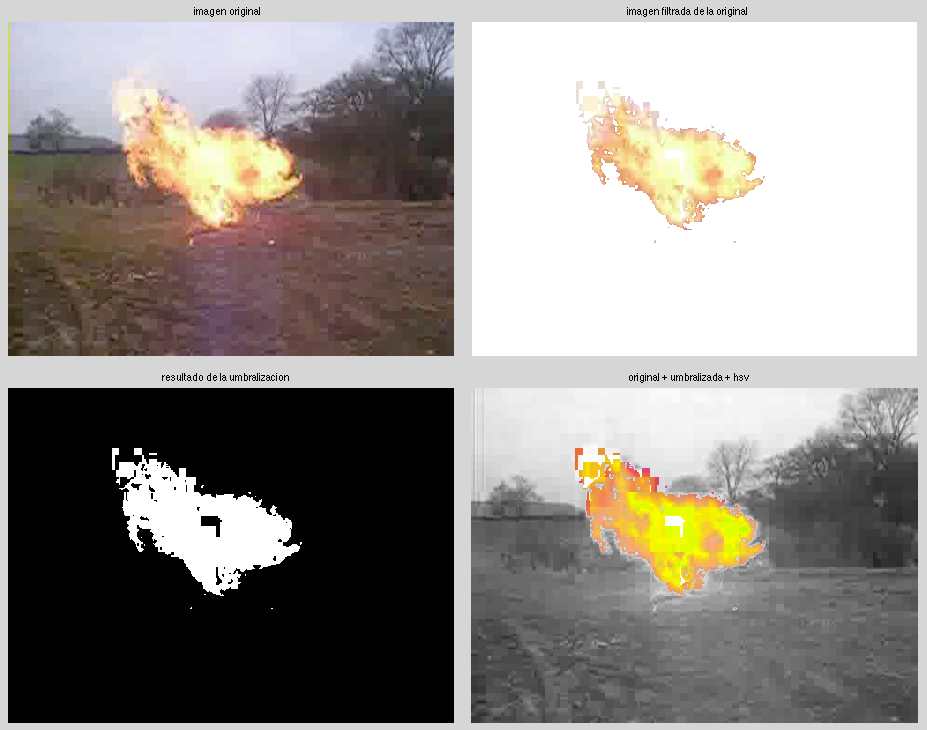
\includegraphics[width=1\textwidth]{img/p7a_fuego.png}
  \caption{Resultados obtenidos en la segmentación de la imagen con fuego.}
  \label{fig:p7a:fuego}
\end{figure}

\begin{figure}[h]
  \centering
    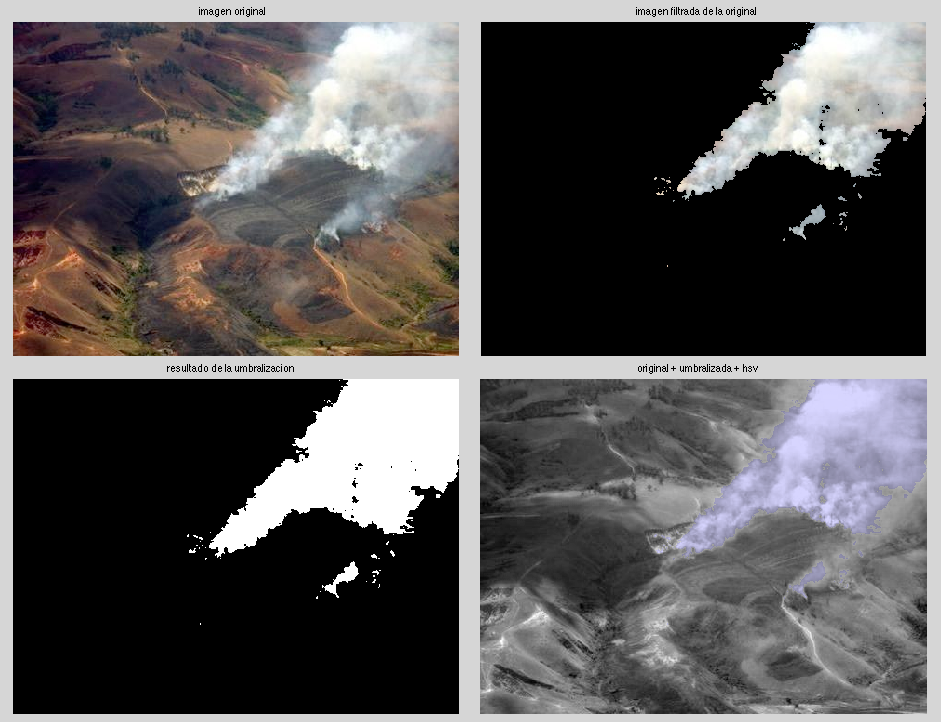
\includegraphics[width=1\textwidth]{img/p7a_humo.png}
  \caption{Resultados obtenidos en la segmentación de la imagen con humo.}
  \label{fig:p7a:humo}
\end{figure}

\subsection{Segundo apartado.}

	Proponer, justificar, diseñar e implementar estrategias que permitan incrementar el nivel de paralelismo obtenido en el primer apartado.
	
\clearpage	

\subsubsection{Implementación.}

	Como en este apartado de la práctica lo que se pide es incrementar el nivel de paralelismo del apartado anterior lo que se ha decidido es tratar cada componente del espacio de colores por separado. Para ello se ha creado un diagrama de flujo para después implementarlo en código tal como el que se puede ver en la figura \ref{fig:p7b:paralelizacion} la fase de paralelización ahorraría mucho tiempo si despreciamos el tiempo que consume el manejo las señales que se añaden para la comunicación de procesos.

\begin{figure}[h]
  \centering
    \includegraphics[width=0.7\textwidth]{img/p7b_paralelizacion.pdf}
  \caption{Diagramas de flujo para el primer apartado y el segundo apartado.}
  \label{fig:p7b:paralelizacion}
\end{figure}

Tanto la entrada como la salida de la FPGA se guardan en tres ficheros distintos, uno para cada componente del espacio de colores. Para guardar las componentes se puede reutilizar la función creada en el apartado anterior (figura \ref{cod:p7a:read_out_FPGA}). Sin embargo para poder leer las imágenes se ha creado una nueva función para dividir la imagen en componentes (véase la figura \ref{cod:p7b:generaEntradaComponentes}).

\begin{figure}[h]
	\begin{lstlisting}[style=matlab]	
%% Esta funcion crea un fichero de texto donde cada linea tiene hay un valor de la matriz de de las componentes
%  parametros
%       inImage  : imagen de entrada
%       nfile    : nombre del archivo de salida
%       component: componente que se quiere guardar
function generaEntradaComponentesFPGA(inImage, nfile, component)

    if (nargin ~= 3)
        error('generaEntradaComponentesFPGA: recibe tres parametros de entrada');
    end
    
    if size(inImage, 3) < component
       error('generaEntradaComponetesFPGA: no existe esa componente'); 
    end

    m = [reshape(inImage(:,:,component), 1, size(inImage, 1) * size(inImage, 2))];
    
    try
        fid = fopen(nfile,'w');
        for i=1:length(m)
            fprintf(fid,'%d ',m(i));
            fprintf(fid,'\r\n'); % salto de linea en windows
        end
        fclose(fid);
    catch
        error('generaEntradaComponentesFPGA: no se ha podido guardar el fichero');
    end
end
	\end{lstlisting}
	\caption{Función \emph{generaEntradaComponentes.m} hecha en matlab Para poder guardar cada componente en un fichero distinto.}
	\label{cod:p7b:generaEntradaComponentes}
\end{figure}	

\subsubsection{Test.}

	Las imágenes obtenidas con la implementación paralela son las mismas que con las versiones secuenciales y se pueden ver en las figuras \ref{fig:p7a:fuego} y \ref{fig:p7a:humo}.

\subsection{Tercer apartado.}

	Para el tercer apartado se pueden escoger a realizar una de dos opciones disponibles, con lo que se ha escogido la opción b que se redacta a continuación.
	
	Aplicar el mecanismo de procesado de imágenes desarrollado en el apartado 1 y dos en otra situación realista mostrando ejemplos de su uso. Justificar la aplicación de una FPGA en dicho problema.
	
\subsubsection{Problema a abordar. Croma.}

	La croma
\footnote{Información obtenida de \url{http://es.wikipedia.org/wiki/Croma}}	
	 o inserción croma es una técnica audiovisual utilizada ampliamente tanto en cine como televisión en incluso en fotografía, que consiste en extraer un color de la imagen y reemplazar el área que ocupaba ese color por otra imagen con la ayuda de un equipo especializado o un ordenador. Esto se hace cuando es demasiado costoso o inviable rodar al personaje en el escenario deseado.
	
	Ningún elemento de la escena debe ser del mismo color de fondo (pues sería eliminado de la imagen), y en vestuario, peluquería, etc se deben evitar los bordes poco definidos, ya que será más difícil ajustar el croma.

\subsubsection{Implementación.}

	Para la implementación de este apartado se a partido de la implementación del apartado 2. Se ha añadido la opción de leer una segunda imagen para establecerla de fondo y en el momento de guardar la imagen lo que se almacena en las posiciones que se ha detectado como croma serán las que están en la imagen de fondo, mientras que lo que no se ha detectado como croma se dejará en la imagen resultante. En la figura \ref{fig:p7c:paralelizacion} se puede ver el diagrama de flujo que se uso para realizar este apartado.

\begin{figure}[h]
  \centering
    
\includegraphics[width=1\textwidth]{img/p7c_paralelizacion.pdf}
  \caption{Diagramas de flujo para el tercer apartado.}
  \label{fig:p7c:paralelizacion}
\end{figure}

\subsubsection{Test.}

	Para probar el código se han seleccionado dos imágenes distintas para probar los resultados. La particularidad de estás imágenes es que el croma que usan no es el mismo y no tienen un color constante, incluso en una de ellas se puede ver los pliegues que hace el croma al no estar colocado de la manera que debía. En las figuras \ref{fig:p7c:test1} y \ref{fig:p7c:tes2} se pueden ver los cromas y los fondos que se emplearon los resultados que se usaron al aplicar los umbrales que aparecen en la tabla \ref{tab:p7c:umbrales}.

\begin{table}
	\begin{center}
		\begin{tabular}{|c|c|c|}
\hline
\textbf{Componente} & \textbf{Mínimo} & \textbf{Máximo} \\ \hline \hline
\textbf{rojo}  &   0 & 110 \\ \hline
\textbf{verde} & 150 & 255 \\ \hline
\textbf{azul}  &   0 &  90 \\ \hline
		\end{tabular}
		\caption{Umbrales para la detección del croma.}
		\label{tab:p7c:umbrales}
	\end{center}
\end{table}

\begin{figure}[h]
  \centering
    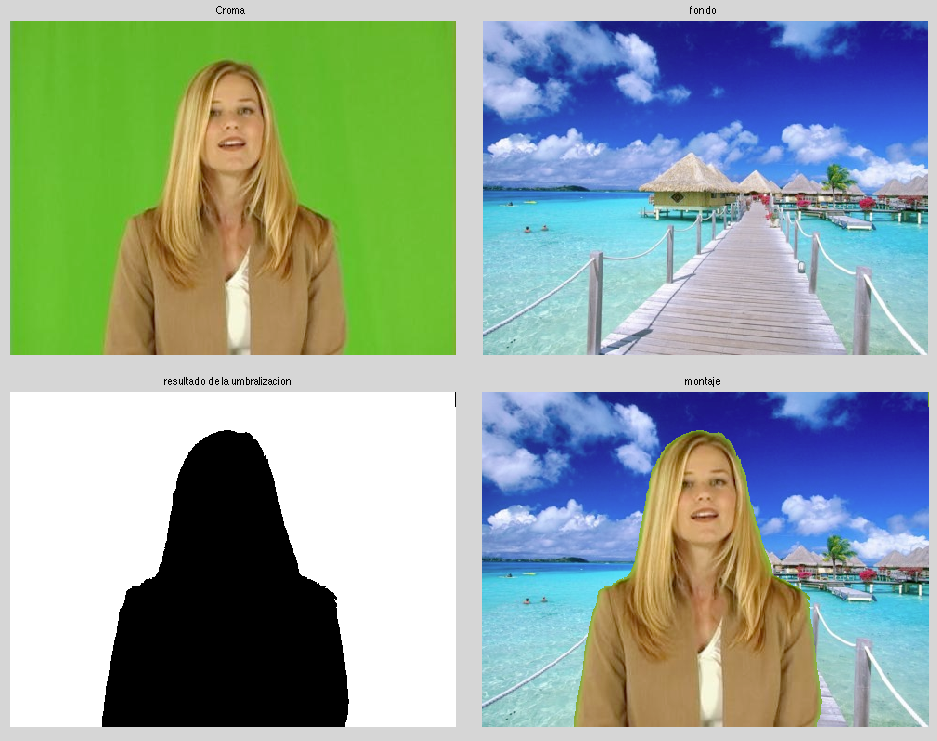
\includegraphics[width=1\textwidth]{img/p7c_test1.png}
  \caption{Resultados obtenidos con el primer croma.}
  \label{fig:p7c:test1}
\end{figure}

\begin{figure}[h]
  \centering
    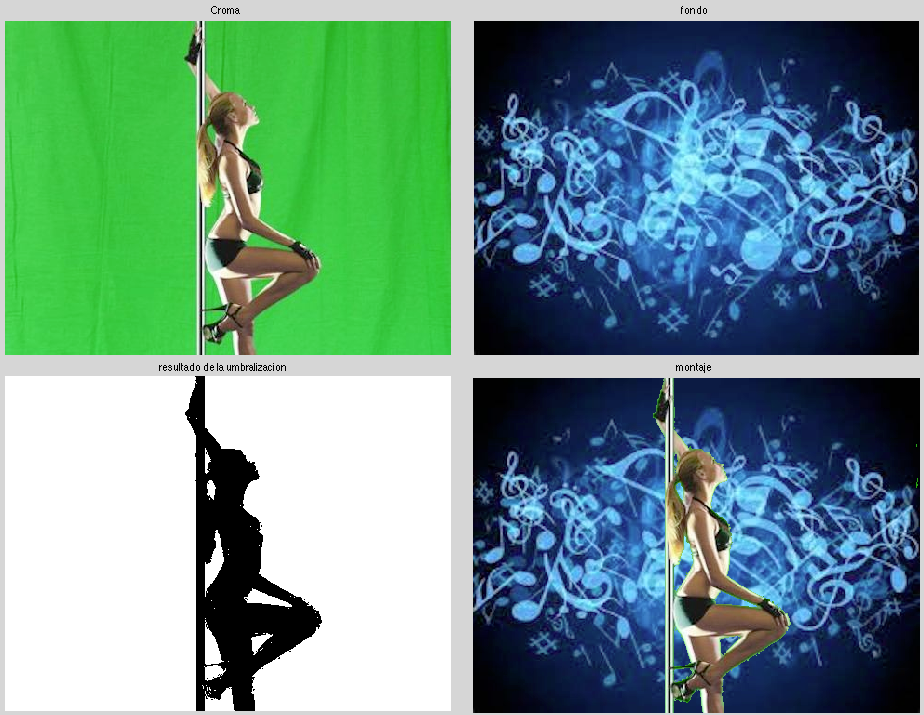
\includegraphics[width=1\textwidth]{img/p7c_test2.png}
  \caption{Resultados obtenidos con el segundo croma.}
  \label{fig:p7c:test2}
\end{figure}

\end{document}